\documentclass{xmum_asg}

\usepackage[english]{babel}
\usepackage{tabularx}
\usepackage{enumitem}
\usepackage{chngcntr}

\setmainfont{Times New Roman}

\graphicspath{{../outputs/figures/}}

\onehalfspacing
\setlength{\parindent}{0pt}
\setlength{\parskip}{6pt}
\setlength{\emergencystretch}{2em}
\setlength{\tabcolsep}{6pt}
\renewcommand{\arraystretch}{1.15}

\captionsetup{font=small,labelfont=bf,labelsep=colon}
\captionsetup[table]{skip=4pt}

\counterwithout{figure}{section}
\counterwithout{table}{section}
\renewcommand{\thefigure}{\arabic{figure}}
\renewcommand{\thetable}{\arabic{table}}
\titleformat{\section}{\fontsize{14}{17}\selectfont\bfseries}{\thesection.}{0.6em}{}
\titlespacing*{\section}{0pt}{18pt}{8pt}
\titleformat{\subsection}{\fontsize{14}{17}\selectfont\bfseries}{\thesubsection}{0.6em}{}
\titlespacing*{\subsection}{0pt}{12pt}{6pt}

\setlist[itemize]{leftmargin=*,itemsep=3pt,topsep=4pt,parsep=0pt}

\hypersetup{pdftitle={Washington's Plug-in Vehicle Population, 2010--2026}}

\begin{document}

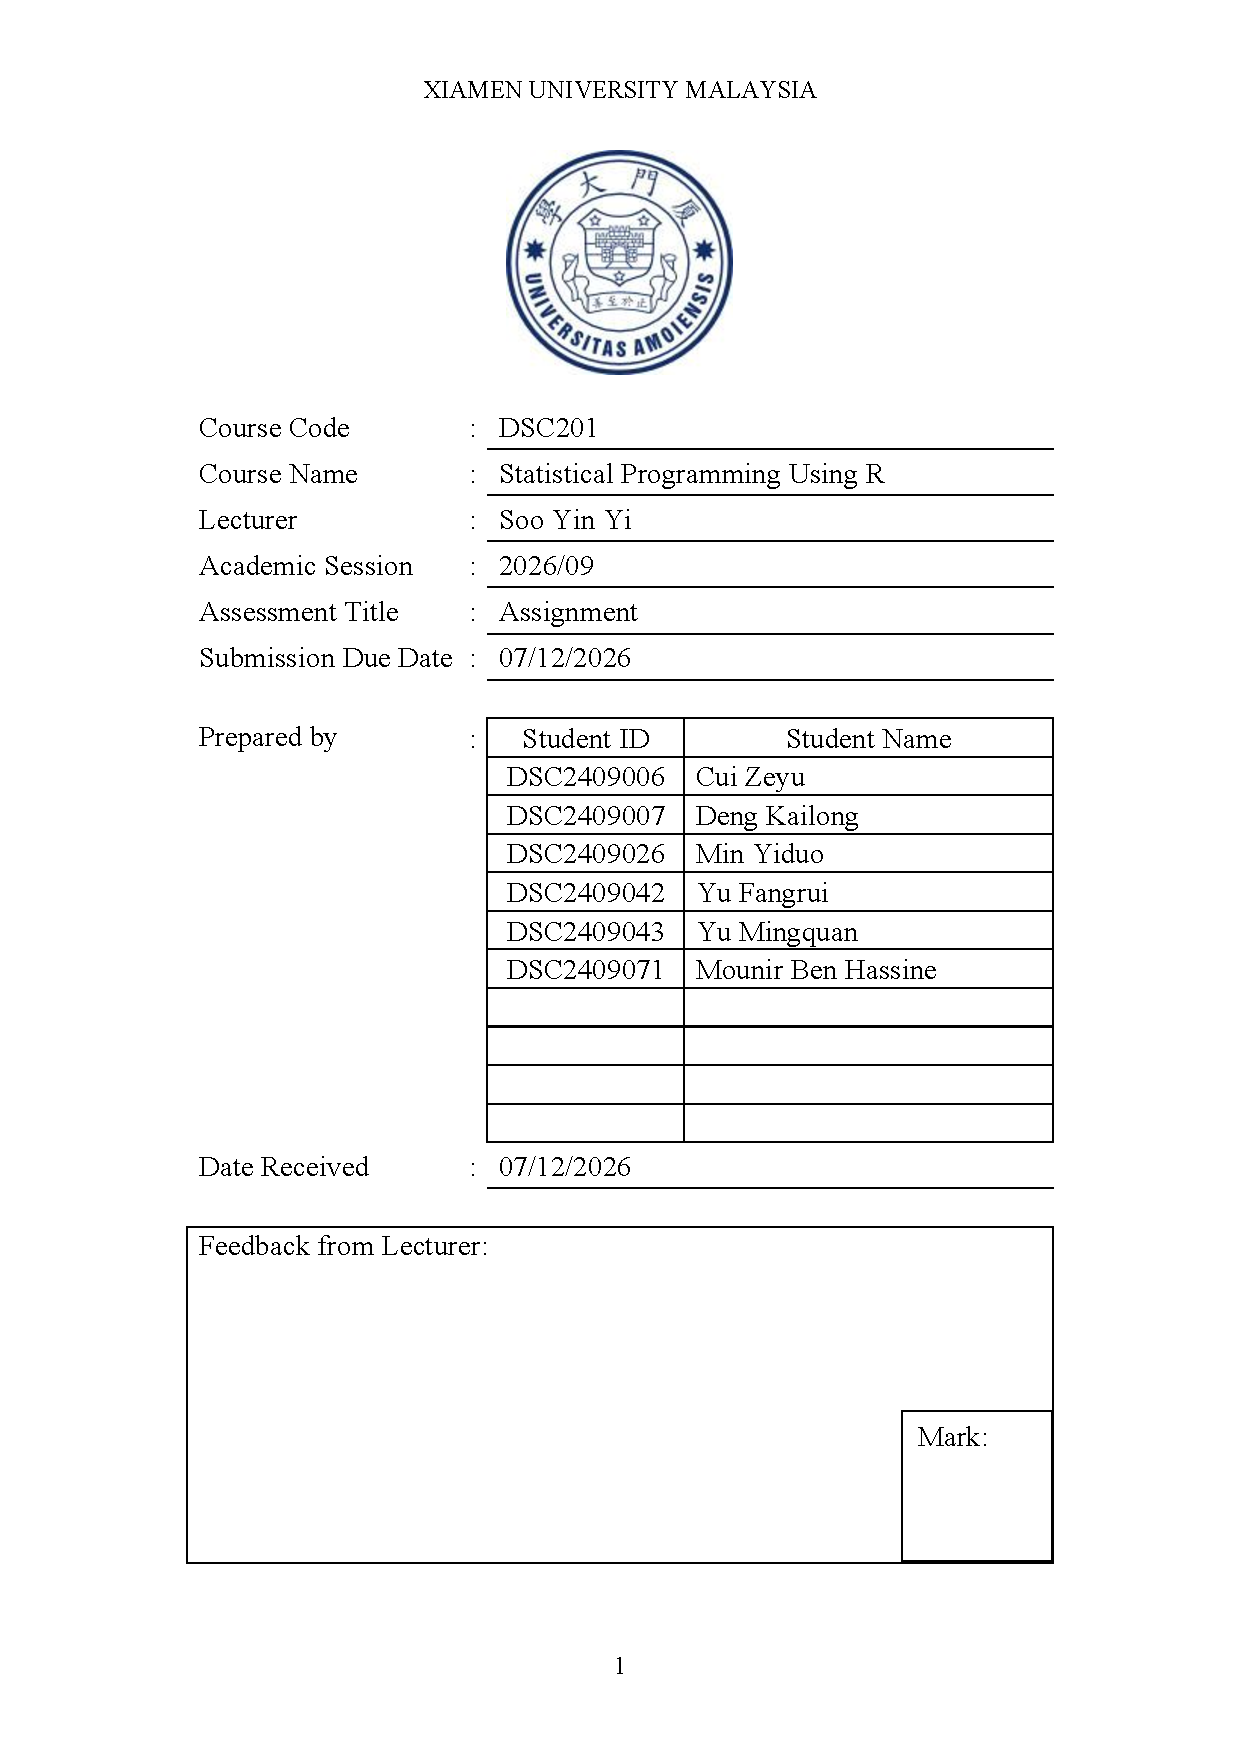
\includepdf[pages=-]{cover_page.pdf}

\pagestyle{empty}
\tableofcontents
\thispagestyle{empty}
\clearpage

\pagestyle{fancy}
\fancyfoot[C]{Page \thepage\ of \pageref{LastMainPage}}
\setcounter{page}{1}

\begin{center}
{\fontsize{14}{17}\selectfont\bfseries Washington's Plug-in Vehicle Population, 2010--2026}
\end{center}

\textbf{Report starter for the team (delete this paragraph before submission).} Bullets only: each group lists the figures and tables to use, the key numbers, where the code is, and what to interpret. Write the prose in your own words. Cite the code as the brief asks, e.g. ``The code for this finding is in sub-section 13.1 of the R code.'' Every number comes from outputs/tables, and every figure from outputs/figures. Wording rules: say ``associated with'', not ``caused by''; a vehicle ``left the records'' (we can't tell whether it moved out of state or went off the road); a used car arriving from elsewhere has its ``first Washington title as used''.

\begin{itemize}
  \item \textbf{Research question:} how has Washington's plug-in vehicle population grown, aged and spread from 2010 to 2026, and which vehicles stay in it? Focus: Population, with Vehicle Specification in support.
\end{itemize}

\section{Context and Data Understanding}

\subsection{The dataset and its context}

\begin{itemize}
  \item \textbf{Source:} Washington State Department of Licensing, ``Electric Vehicle Title and Registration Activity'', data.wa.gov, dataset ID rpr4-cgyd, licence ODbL. Extract of 7 November 2026 (source updated 14 October 2026); frozen by SHA-256 so results can be reproduced.
  \item \textbf{Size:} 1,926,507 rows, 33 columns, 401,956 distinct vehicles, January 2010 to September 2026.
  \item \textbf{Type of data:} administrative transaction records, not a survey. One row = one transaction: original title, transfer title, original registration, renewal, registration at transfer.
  \item \textbf{Variables (feature groups):} vehicle (VIN prefix, make, model, model year, BEV/PHEV type, electric range); transaction (type, date, sale price, sale date, odometer, New/Used label); location (county, city, postal code, 2020 census tract, legislative district, electric utility); policy fields (2019 HB 2042 tax-exemption eligibility, EV fees paid).
  \item \textbf{Measurement characteristics to mention:} prices exist only on title rows; a new car's registration row says ``Used'' (worked example in sub-section 2.3); electric range is almost missing for BEVs after model year 2020; the population is not given directly and has to be rebuilt from the transactions.
  \item \textbf{Supporting data:} US Census Bureau county population estimates (per-resident rates, section 19) and BLS CPI-U (real prices, section 7).
  \item \textbf{code: sections 1--2 (data dictionary: 2.1; transaction types: 2.5).}
  \item \textbf{Table to use:} 02\_data\_dictionary.csv (source description and profile of every column) --- summarise it as a short variable table, not all 33 rows.
\end{itemize}

\subsection{Indicators that summarise the population}

\begin{itemize}
  \item \textbf{Derived indicators:} active vehicles per year, entries (first Washington record), exits (no record for two years), returns, vehicle age, BEV share, county share, entry route (new, first Washington title as used, registration only), county moves.
\end{itemize}

\begin{figure}[H]
\centering
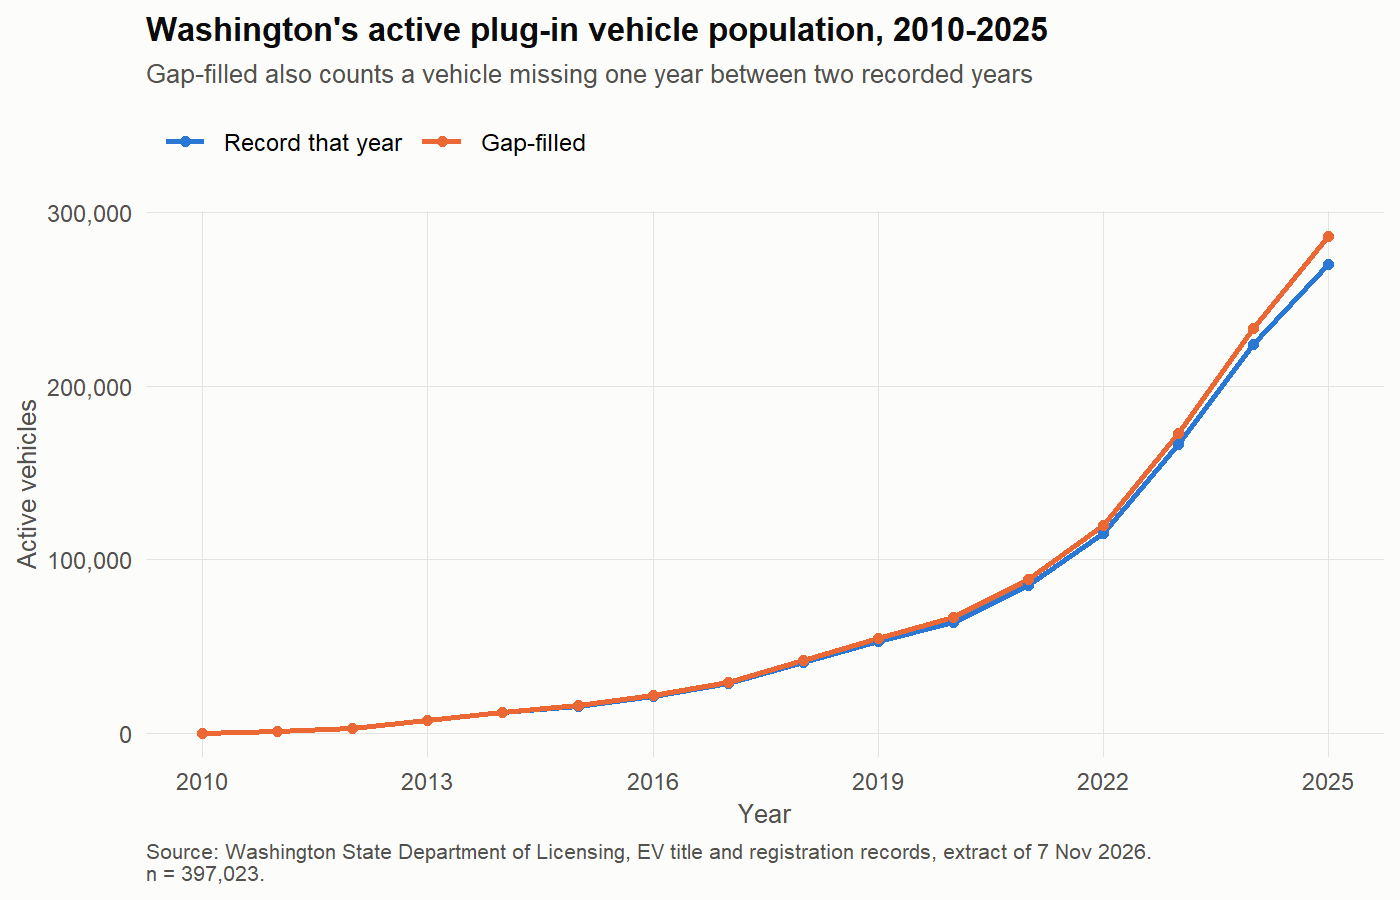
\includegraphics[width=6in,height=0.85\textheight,keepaspectratio]{11_01_active_population.png}
\caption{Active plug-in vehicles per year, simple and gap-filled counts (11\_01\_active\_population.png)}
\end{figure}

\begin{table}[htbp]
\centering
\small
\setlength{\tabcolsep}{5pt}
\caption{Population stock and flows by year (06\_population\_flows.csv)}
\begin{tabular}{rrrrrrr}
\toprule
\textbf{Year} & \textbf{Active (simple)} & \textbf{Active (gap-filled)} & \textbf{Entries} & \textbf{Leavers after year} & \textbf{BEV \%} & \textbf{Mean age}\\
\midrule
2010 & 80 & 80 & 80 & 4 & 97.5 & 3.79\\
2011 & 1,177 & 1,179 & 1,103 & 56 & 88.4 & 0.35\\
2012 & 2,932 & 2,958 & 1,835 & 104 & 62.9 & 0.5\\
2013 & 7,528 & 7,623 & 4,769 & 473 & 69.9 & 0.59\\
2014 & 11,821 & 12,125 & 4,973 & 942 & 69.4 & 1.04\\
2015 & 15,695 & 16,230 & 5,043 & 1,427 & 69.6 & 1.48\\
2016 & 20,973 & 21,716 & 6,895 & 1,830 & 66 & 1.89\\
2017 & 28,485 & 29,436 & 9,508 & 2,284 & 65.6 & 2.21\\
2018 & 40,746 & 42,131 & 14,913 & 3,046 & 66.2 & 2.26\\
2019 & 52,710 & 54,733 & 15,554 & 3,615 & 69.2 & 2.58\\
2020 & 63,724 & 66,708 & 15,492 & 4,360 & 71.7 & 2.92\\
2021 & 85,340 & 88,867 & 26,248 & 6,359 & 73.4 & 2.97\\
2022 & 114,914 & 119,640 & 36,674 & 7,940 & 76.2 & 2.9\\
2023 & 166,427 & 173,070 & 60,788 & 12,539 & 78 & 2.67\\
2024 & 224,133 & 233,487 & 72,036 & 20,215 & 79.1 & 2.76\\
2025 & 270,098 & 286,478 & 71,635 & 95,537 & 79.8 & 3.05\\
2026 & 242,352 & 242,352 & 49,477 &  & 80.6 & 3.55\\
\bottomrule
\end{tabular}
\end{table}

\begin{itemize}
  \item \textbf{Key numbers:} 52,710 active vehicles in 2019 and 270,098 in 2025 (54,733 and 286,478 when a one-year gap is filled). Entries rose from 15,554 (2019) to 60,788 (2023) and about 72,000 a year in 2024--2025. BEV share 69.2\% $\rightarrow$ 79.8\%; mean age 2.58 $\rightarrow$ 3.05 years (2019 $\rightarrow$ 2025).
  \item \textbf{Interpret:} five-fold growth in six years; the fleet is getting older as well as larger; 2024 and 2025 leaver counts are provisional because later years are partial (say so).
  \item \textbf{code: sections 4--6 (definitions), 6 (flows table), 11.1 (figure).}
\end{itemize}

\subsection{Variability, distributions and correlation}

\begin{figure}[H]
\centering
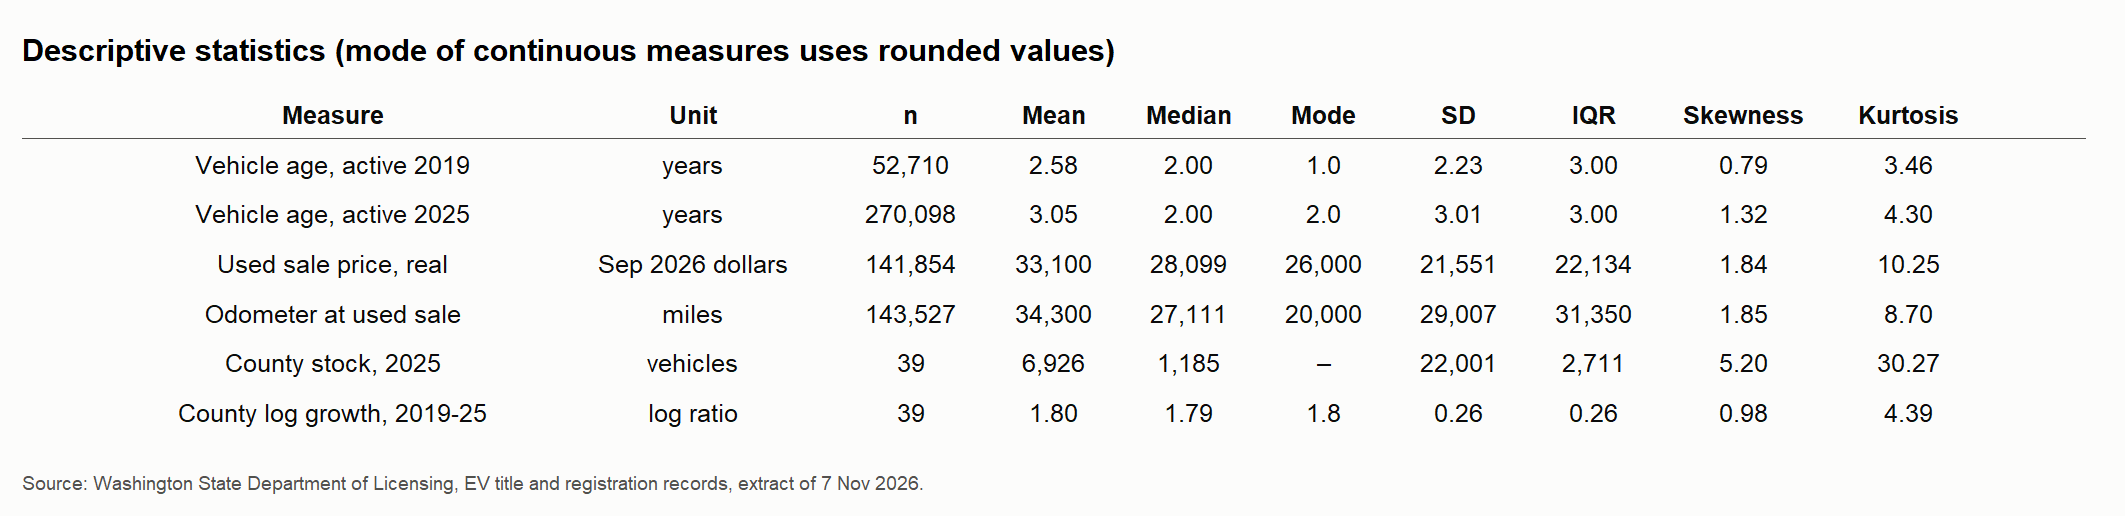
\includegraphics[width=6in,height=0.85\textheight,keepaspectratio]{10_05_table_descriptives.png}
\caption{Descriptive statistics: mean, median, mode, variance, SD, skewness, kurtosis (10\_05\_table\_descriptives.png)}
\end{figure}

\begin{itemize}
  \item \textbf{Vehicle age, 2025:} mean 3.05, median 2, mode 2 years, SD 3.01, skewness 1.32, excess kurtosis 1.30 (right-skewed: many young cars, a long tail of old ones). 2019: mean 2.58, SD 2.23.
  \item \textbf{Real used sale price:} mean \$33,100, median \$28,099, SD \$21,551, skewness 1.84, kurtosis 10.3 (141,854 used sales, September 2026 dollars). Use the median as the typical value.
  \item \textbf{County stock, 2025:} mean 6,926 but median 1,185; skewness 5.2, because King alone has 134,140 vehicles.
\end{itemize}

\begin{figure}[H]
\centering
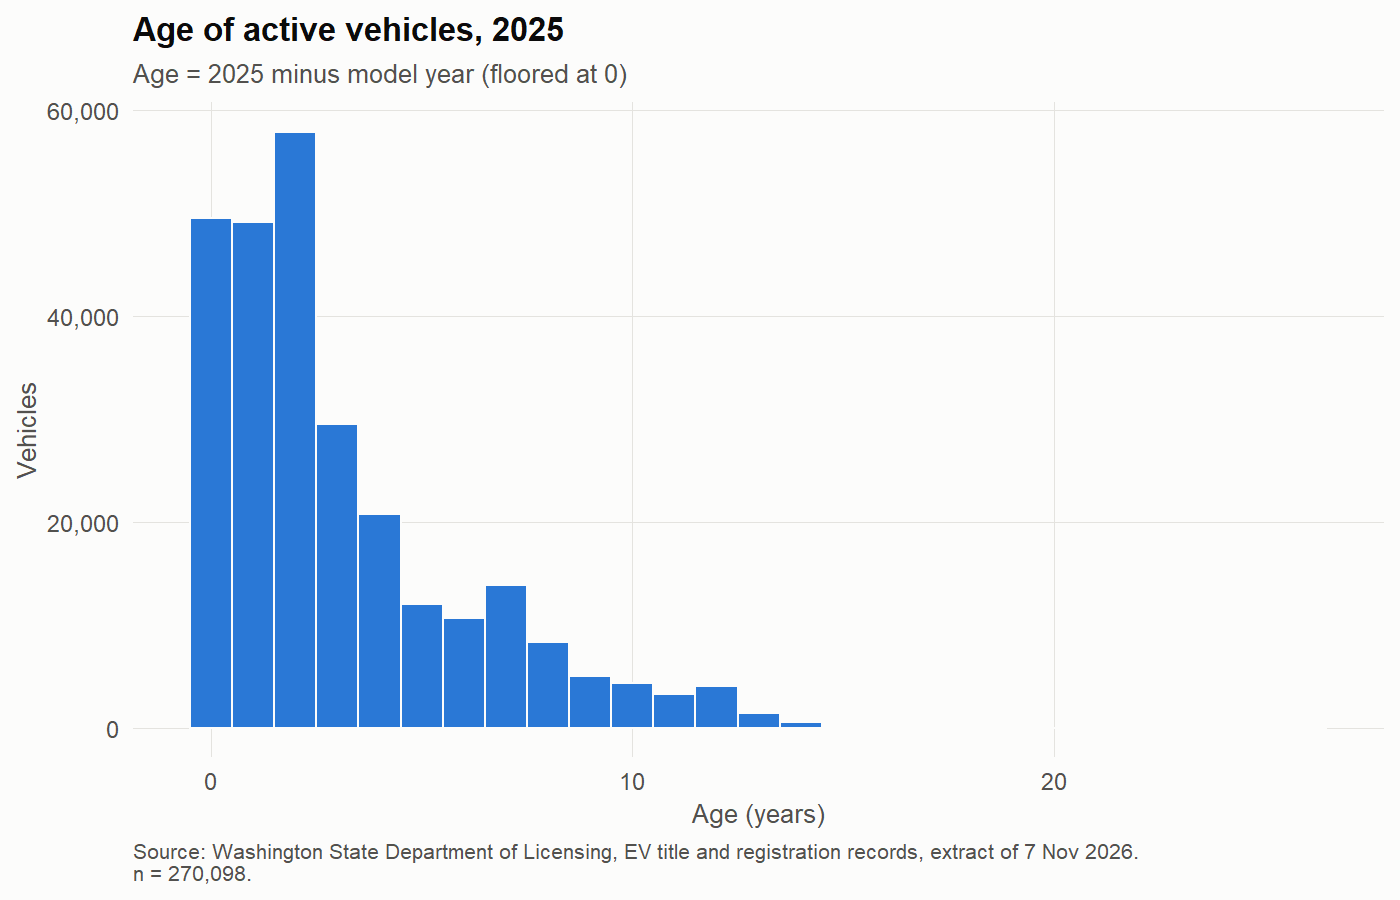
\includegraphics[width=6in,height=0.85\textheight,keepaspectratio]{11_07_age_histogram_2025.png}
\caption{Distribution of vehicle age, 2025 (11\_07\_age\_histogram\_2025.png)}
\end{figure}

\begin{figure}[H]
\centering
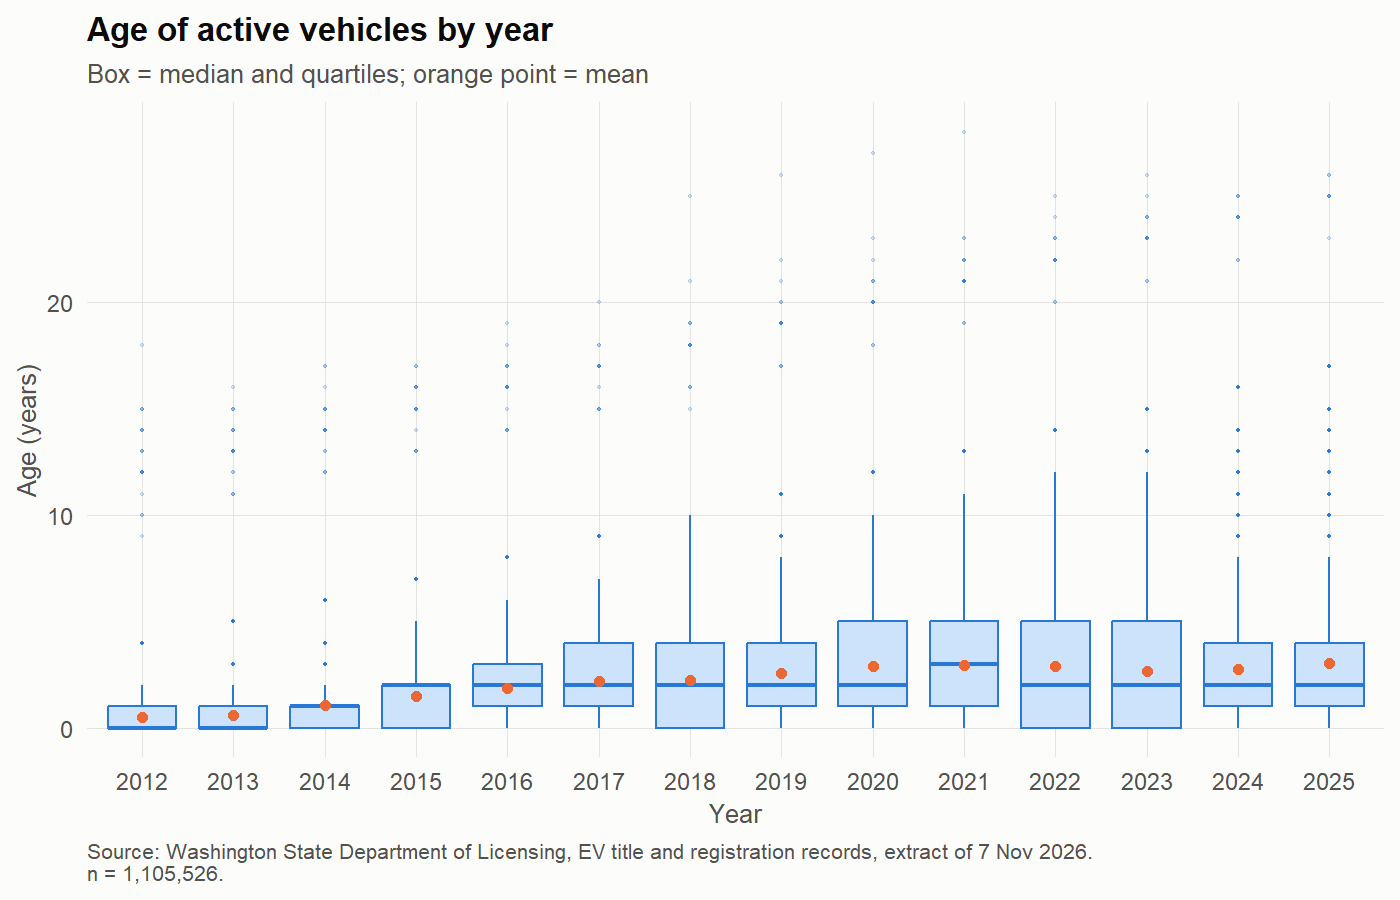
\includegraphics[width=6in,height=0.85\textheight,keepaspectratio]{11_09_age_by_year_boxplot.png}
\caption{Vehicle age by year (boxplots) (11\_09\_age\_by\_year\_boxplot.png)}
\end{figure}

\begin{figure}[H]
\centering
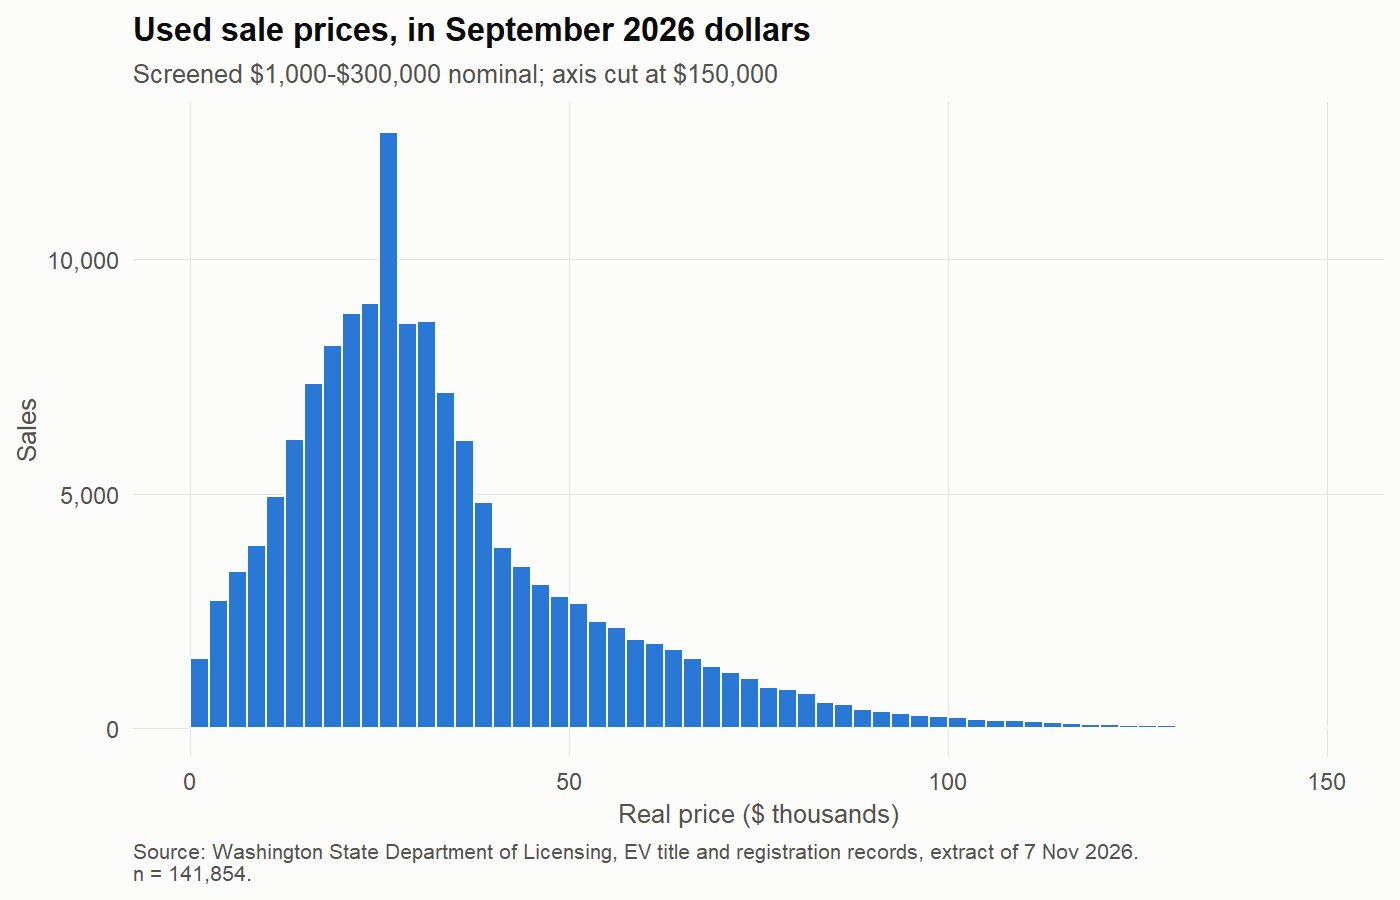
\includegraphics[width=6in,height=0.85\textheight,keepaspectratio]{11_08_used_price_histogram.png}
\caption{Distribution of real used sale prices (11\_08\_used\_price\_histogram.png)}
\end{figure}

\begin{figure}[H]
\centering
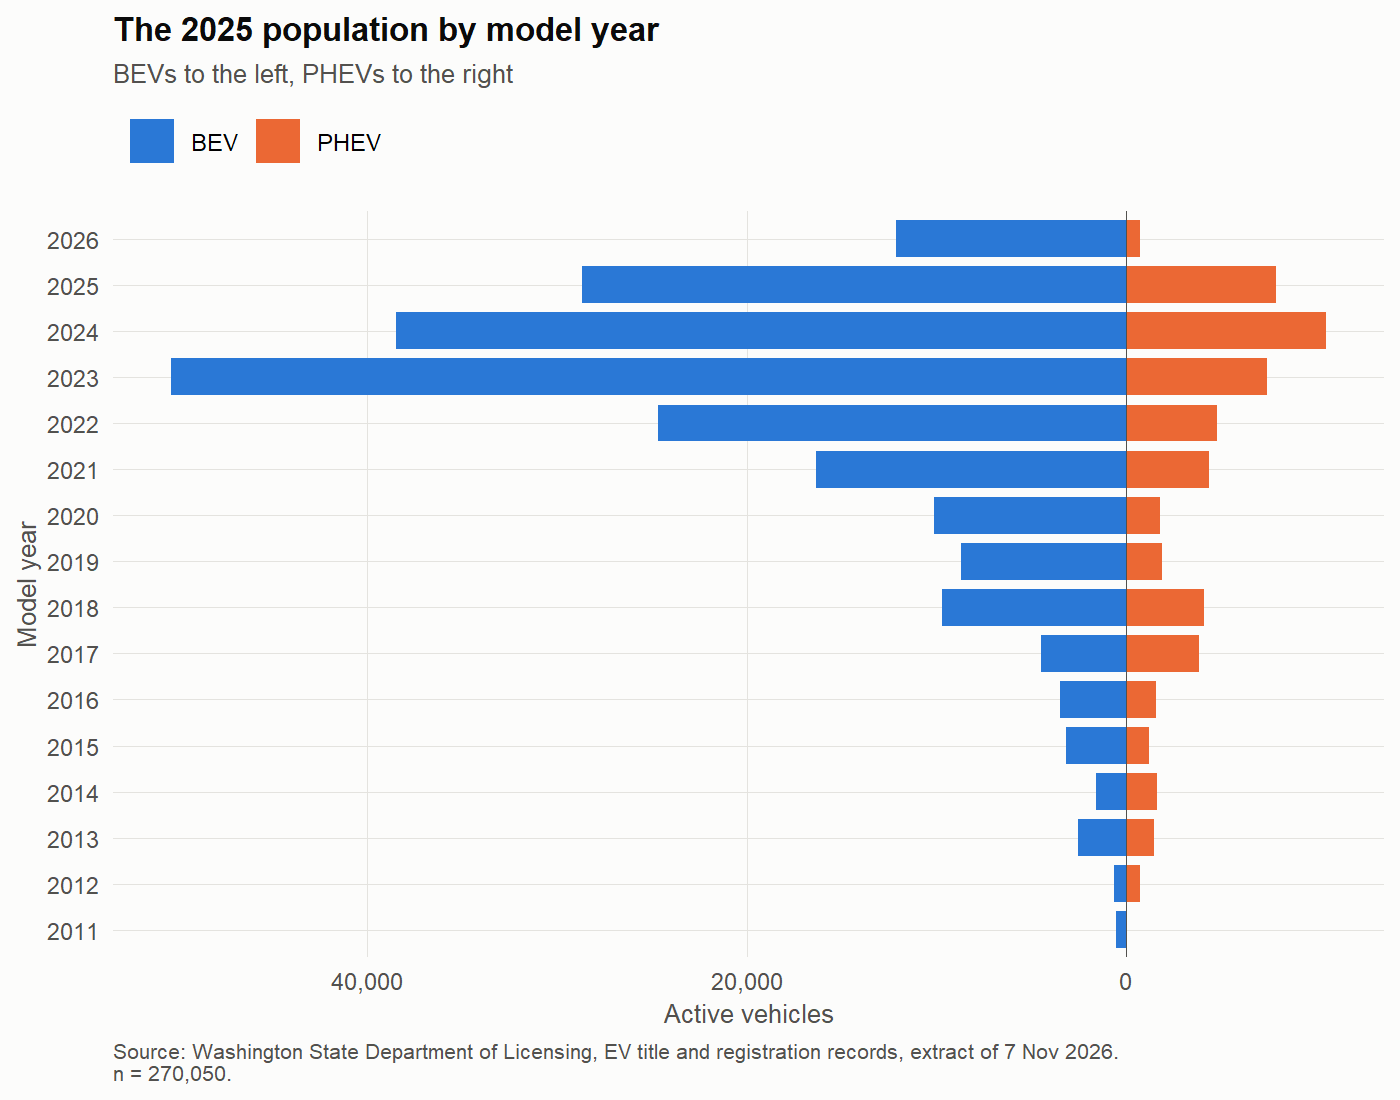
\includegraphics[width=6in,height=0.85\textheight,keepaspectratio]{11_12_model_year_pyramid_2025.png}
\caption{Active vehicles in 2025 by model year and type (11\_12\_model\_year\_pyramid\_2025.png)}
\end{figure}

\begin{itemize}
  \item \textbf{Correlation (39 counties):} growth 2019--25 vs log 2019 stock: Pearson r = $-0.31$ (p = 0.058), Spearman $-0.33$, Kendall $-0.22$ --- smaller counties grew slightly faster (weak). Growth vs used share in 2019: r = 0.42 (p = 0.008).
  \item \textbf{Correlation (used sales):} log real price vs age r = $-0.66$; vs odometer r = $-0.49$; age vs odometer r = 0.69 (older cars have more miles, so the two overlap).
  \item \textbf{Interpret:} skewed variables $\rightarrow$ report medians and use logs; Pearson and Spearman agree in direction; correlation shows association only.
  \item \textbf{code: 10.3 (county measures), 10.4 (descriptives: 10\_descriptives.csv), 10.5 (10\_correlations.csv), 11.7--11.9, 11.12.}
\end{itemize}

\subsection{Which vehicles, and where}

\begin{figure}[H]
\centering
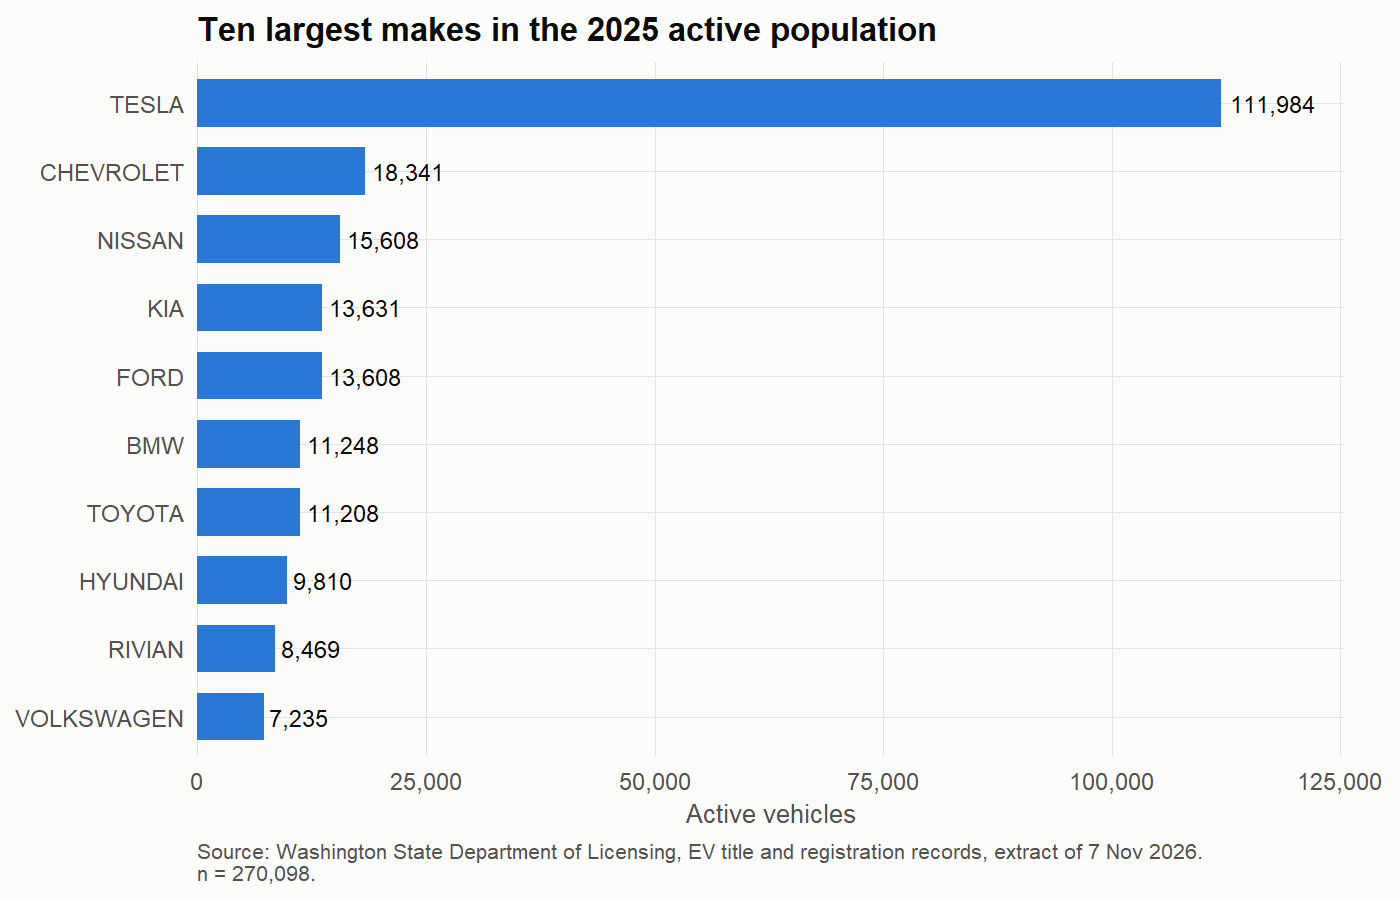
\includegraphics[width=6in,height=0.85\textheight,keepaspectratio]{11_05_top_makes_2025.png}
\caption{Top makes among active vehicles, 2025 (11\_05\_top\_makes\_2025.png)}
\end{figure}

\begin{figure}[H]
\centering
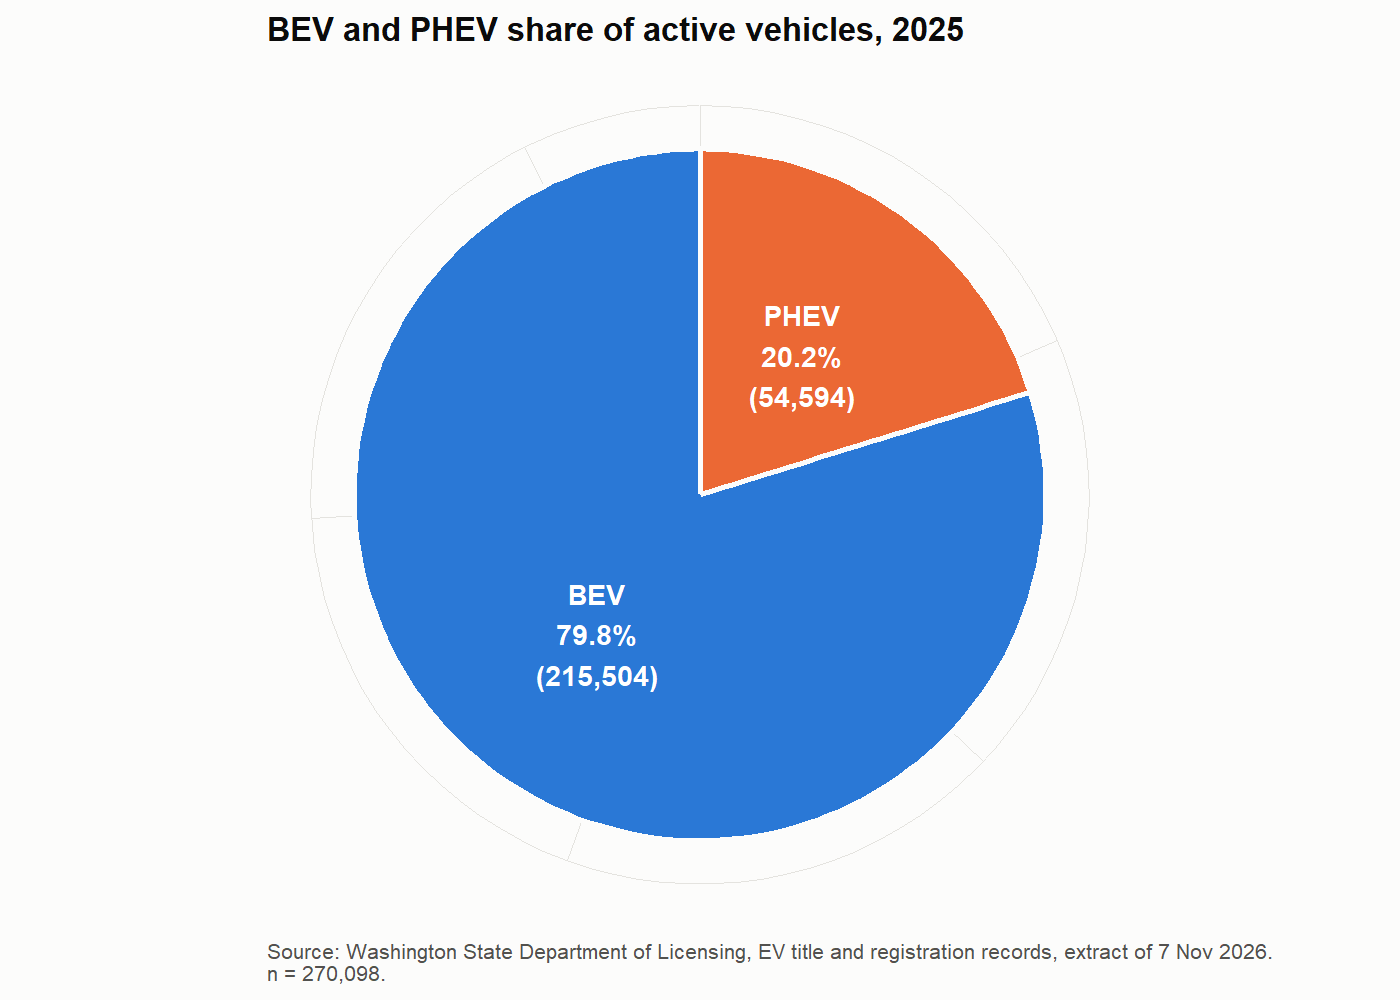
\includegraphics[width=5.2in,height=0.85\textheight,keepaspectratio]{11_06_type_share_2025.png}
\caption{BEV and PHEV share of active vehicles, 2025 (11\_06\_type\_share\_2025.png)}
\end{figure}

\begin{figure}[H]
\centering
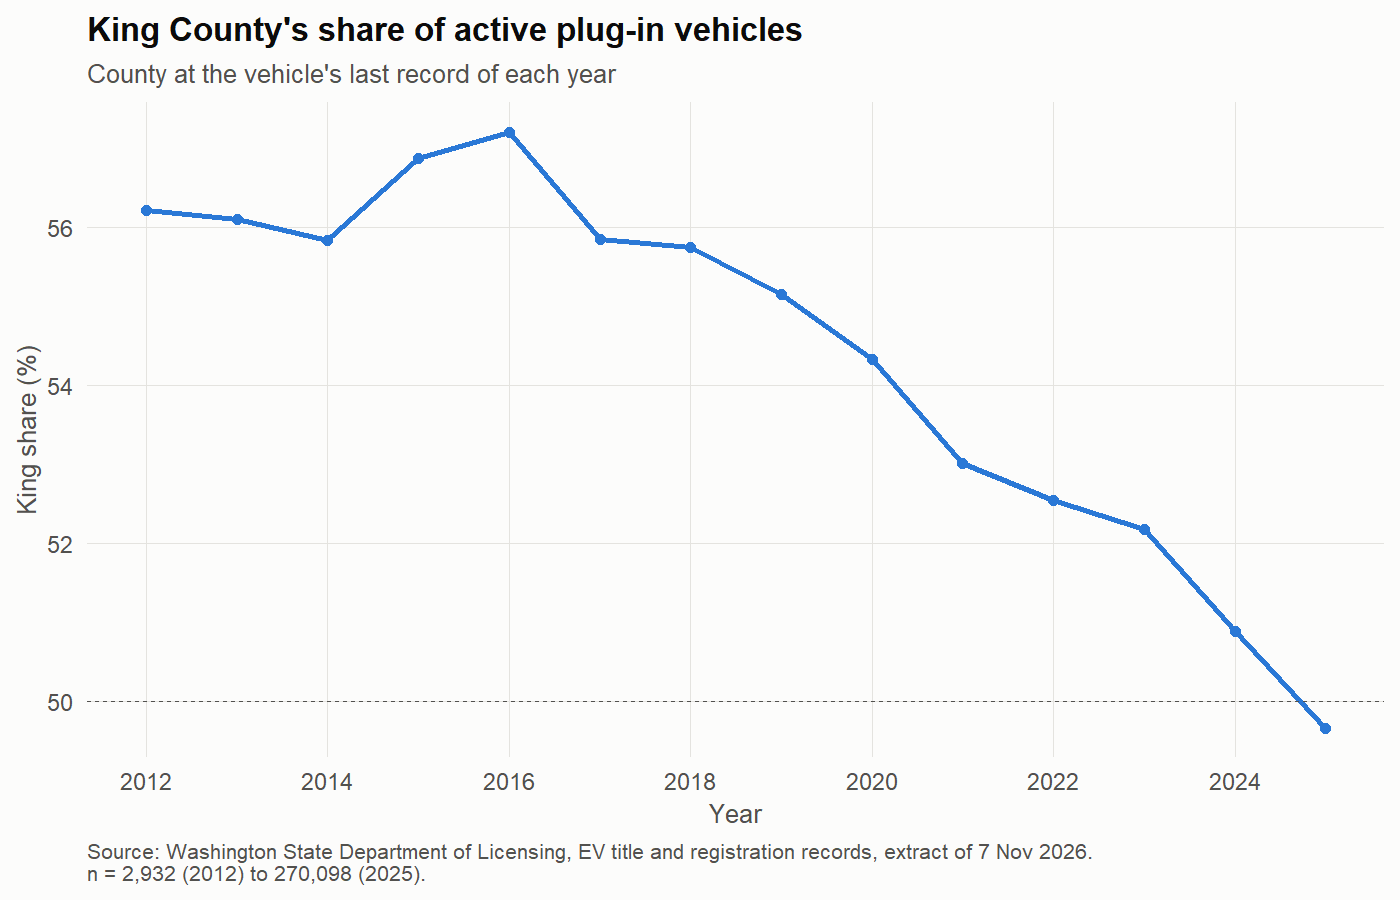
\includegraphics[width=6in,height=0.85\textheight,keepaspectratio]{11_02_king_share.png}
\caption{King County's share of active vehicles (11\_02\_king\_share.png)}
\end{figure}

\begin{figure}[H]
\centering
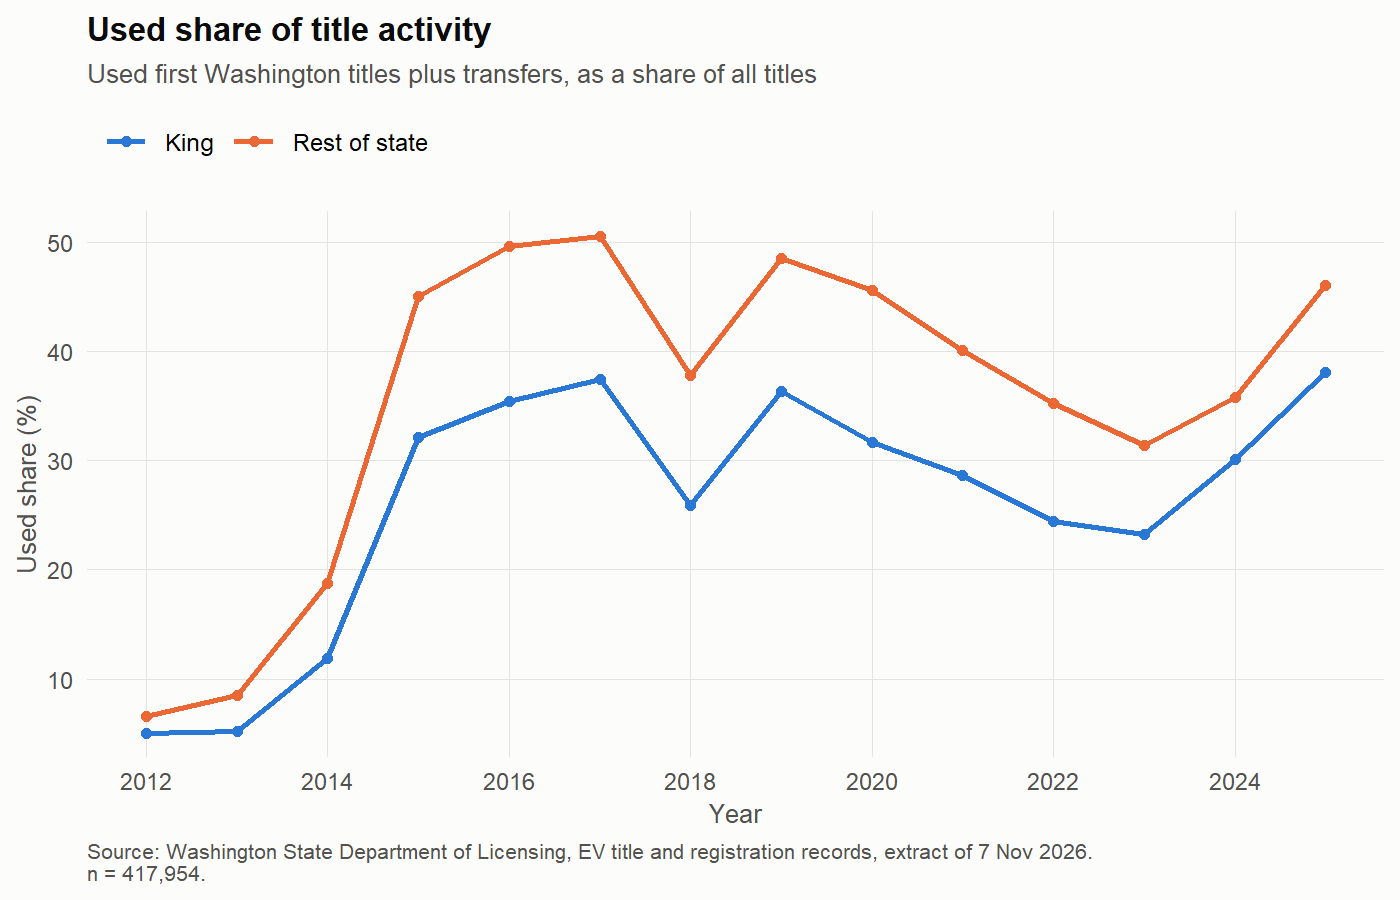
\includegraphics[width=6in,height=0.85\textheight,keepaspectratio]{11_03_used_share.png}
\caption{Used share of title activity, King and the rest of the state (11\_03\_used\_share.png)}
\end{figure}

\begin{figure}[H]
\centering
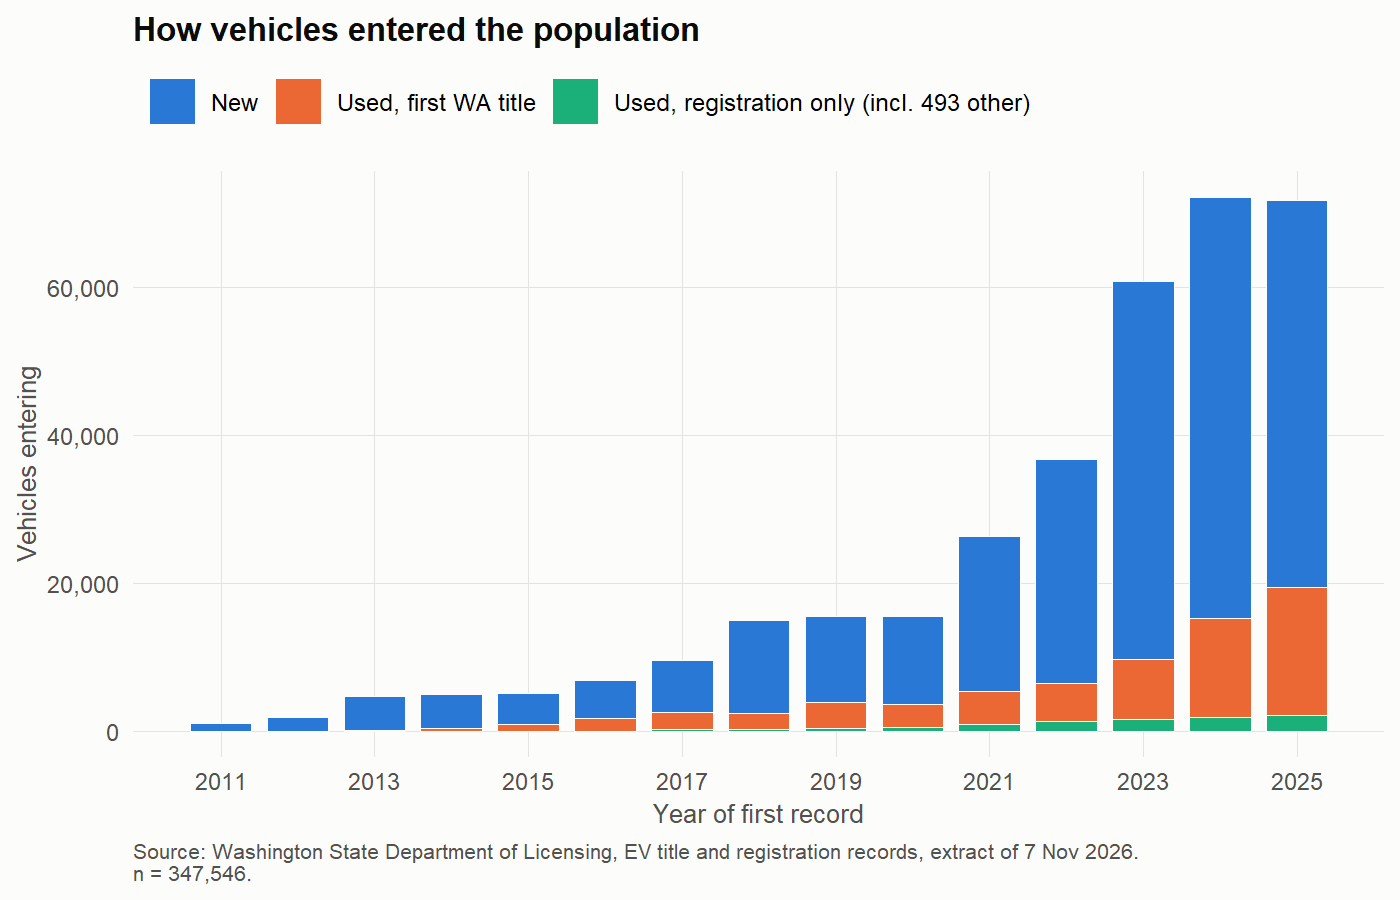
\includegraphics[width=6in,height=0.85\textheight,keepaspectratio]{11_04_entry_routes.png}
\caption{How vehicles first enter the Washington records, by year (11\_04\_entry\_routes.png)}
\end{figure}

\begin{itemize}
  \item \textbf{Frequency tables (as PNG and CSV):} 10\_01 vehicles by year and type, 10\_02 makes, 10\_03 counties, 10\_04 entry routes.
  \item \textbf{Key numbers:} King's share of active vehicles fell from 55.1\% (2019) to 49.7\% (2025).
  \item \textbf{code: 10.2 (frequency tables), 11.2--11.6.}
\end{itemize}

\section{Data Pre-processing}

\subsection{Import checks}

\begin{itemize}
  \item Raw file verified by SHA-256 and row count before use; every column read as text, then parsed with explicit checks (dates, model year, price): the script stops if any value fails to parse.
  \item Date parsing forced to English month names (otherwise every date becomes missing on a non-English computer, with no error).
  \item \textbf{code: sections 1--2.}
\end{itemize}

\subsection{Cleaning rules, step by step}

\begin{table}[htbp]
\centering
\footnotesize
\caption{Records kept at each cleaning step (09\_flow\_table.csv)}
\begin{tabularx}{\textwidth}{@{}XrrrX@{}}
\toprule
\textbf{Step} & \textbf{Rows} & \textbf{Vehicles} & \textbf{Rows removed} & \textbf{Reason}\\
\midrule
Raw file & 1,926,507 & 401,956 & & \\
Remove exact duplicate rows & 1,926,431 & 401,956 & 76 & \\
Remove hydrogen vehicles & 1,926,381 & 401,935 & 50 & \\
Keep Washington addresses with a county & 1,918,148 & 401,256 & 8,233 & \\
Remove exempt use classes & 1,909,358 & 397,082 & 8,790 & No annual renewal, so exit can't be measured\\
Remove low-speed and off-road classes & 1,909,074 & 397,023 & 284 & Not general road vehicles\\
Vehicle-years & 1,349,135 & 397,023 & & \\
Vehicle histories & 397,023 & 397,023 & & \\
\bottomrule
\end{tabularx}
\end{table}

\begin{itemize}
  \item \textbf{Duplicates:} 76 exact duplicate rows removed (all 33 columns identical).
  \item \textbf{Out of scope:} hydrogen vehicles (not plug-in), records without a Washington address and county, exempt use classes (no annual renewal, so leaving can't be measured), low-speed and off-road classes.
  \item \textbf{Result:} 1,909,074 rows and 397,023 vehicles in the study population.
\end{itemize}

\begin{table}[htbp]
\centering
\small
\caption{How much each rule changes the headline numbers (09\_rule\_effects.csv)}
\begin{tabularx}{\textwidth}{@{}Xrrr@{}}
\toprule
\textbf{After rule} & \textbf{Vehicles ever} & \textbf{Active 2025} & \textbf{King share 2025 (\%)}\\
\midrule
After removing duplicates & 401,956 & 271,965 & 49.47\\
After removing hydrogen & 401,935 & 271,957 & 49.47\\
After keeping Washington addresses & 401,256 & 270,909 & 49.69\\
After removing exempt classes & 397,082 & 270,142 & 49.66\\
After removing low-speed classes (study population) & 397,023 & 270,098 & 49.67\\
Sensitivity: passenger class only & 383,262 & 259,792 & 49.94\\
\bottomrule
\end{tabularx}
\end{table}

\begin{itemize}
  \item \textbf{Interpret:} the rules change active vehicles in 2025 by under 1\% and King's share by under 0.3 points, so no conclusion depends on them.
  \item \textbf{code: section 3; rule effects 9.3.}
\end{itemize}

\subsection{Inconsistencies corrected}

\begin{itemize}
  \item \textbf{New/Used label:} 305,781 of 310,820 new-car titles have a same-day registration labelled ``Used''; entry route is therefore taken from the title, not the label (2.3, 5.1).
  \item \textbf{Several counties in one year:} 13,677 vehicle-years; the county at the last record of the year is used, so county totals add up to the state total (4, 9.2).
  \item \textbf{Fields that should never change for a vehicle} (type, model year, make, model): checked, and none changes (2.4).
  \item \textbf{Prices:} 17 prices whose digits are the sale date (e.g. \$62,720 on 27/06/2020) removed; range kept to \$1,000--\$300,000; 23 same-day conflicting prices set aside; prices converted to September 2026 dollars with CPI-U (October 2025 has no CPI, so those sales drop out).
\end{itemize}

\begin{table}[htbp]
\centering
\small
\caption{Price records kept at each step (07\_price\_flow.csv)}
\begin{tabularx}{\textwidth}{@{}Xr@{}}
\toprule
\textbf{Step} & \textbf{Rows}\\
\midrule
Title rows & 483,815\\
Price recorded & 428,759\\
Sale date recorded & 428,759\\
Not date-like & 428,742\\
\$1,000 to \$300,000 & 427,500\\
After removing same-day conflicts (sale events) & 427,420\\
With CPI (excludes October 2025) & 423,221\\
Used sale events & 144,240\\
Used sale events in the mileage sample & 143,527\\
\bottomrule
\end{tabularx}
\end{table}

\begin{itemize}
  \item \textbf{Mileage:} odometer readings kept as a separate sample with their own checks (07\_odometer\_checks.csv).
  \item \textbf{code: 2.3--2.4, 4, 5.1, 7.1--7.6.}
\end{itemize}

\subsection{Feature engineering}

\begin{itemize}
  \item \textbf{From transactions to a population:} 1,349,135 vehicle-year records (one per vehicle per year) and one history per vehicle (first and last year, entry route, transfers, moves).
  \item \textbf{Exit rule:} no record in the next two years; a vehicle that comes back later is a ``return''. A gap-filled count treats a one-year gap as still active.
  \item \textbf{Other features:} age, tenure in the records, prior transfers, region (King / Western / Eastern Washington), county size class, real price.
  \item \textbf{code: sections 4--6.}
\end{itemize}

\subsection{Verification}

\begin{figure}[H]
\centering
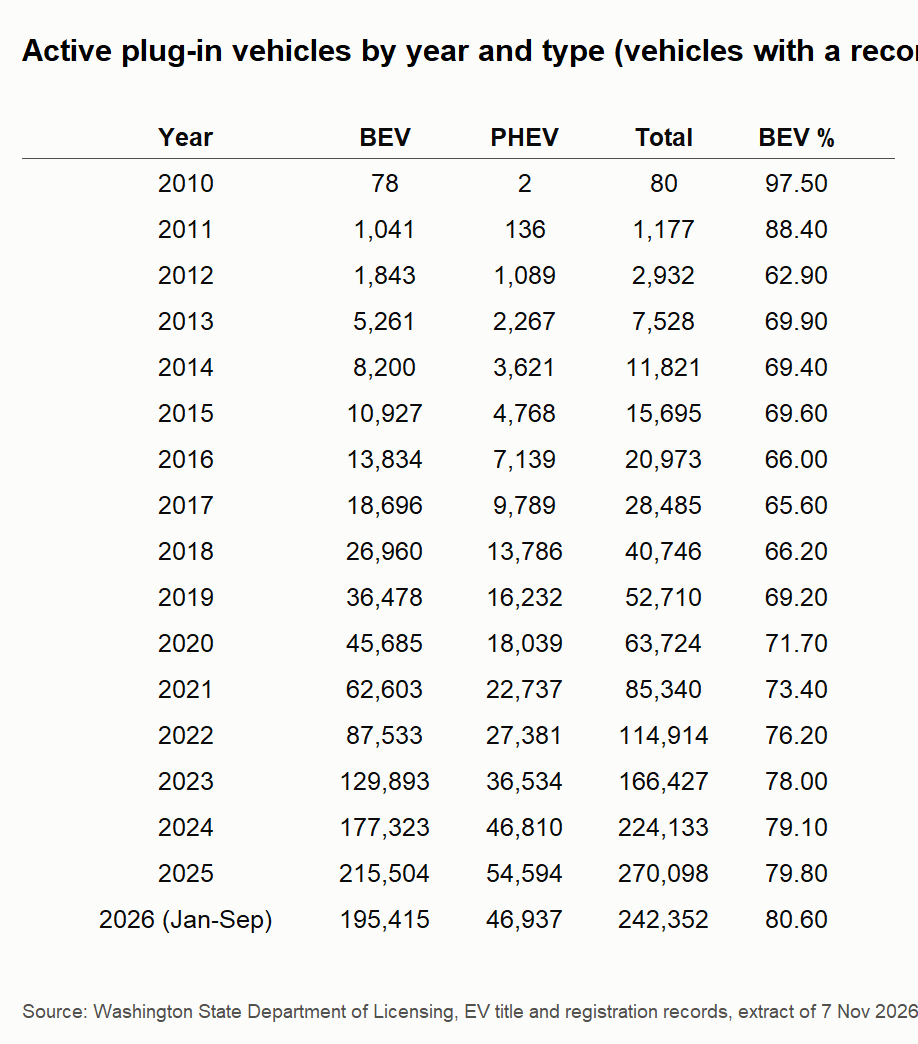
\includegraphics[width=6in,height=0.85\textheight,keepaspectratio]{10_01_table_vehicles_by_year_type.png}
\caption{Vehicles by year and type (frequency table) (10\_01\_table\_vehicles\_by\_year\_type.png)}
\end{figure}

\begin{itemize}
  \item \textbf{Stock and flow reconcile exactly:} active next year = active + entries + returns $-$ leavers, for every year (9.1).
  \item \textbf{Independent cross-check:} 70 benchmark figures computed separately from the data portal (data.wa.gov) were recomputed; 66 match exactly or to rounding, and the 4 differences are explained (09\_benchmark\_cross\_check.csv).
  \item \textbf{Hand check:} ten vehicle histories across the main cases (09\_hand\_check\_vehicles.csv).
  \item \textbf{Limits:} leaving is inferred from missing records; the 2025 count is slightly provisional; 2026 is partial (to 30 September).
  \item \textbf{code: section 9.}
\end{itemize}

\section{Statistical Analysis and Modeling}

\subsection{Probability and distributions}

\begin{figure}[H]
\centering
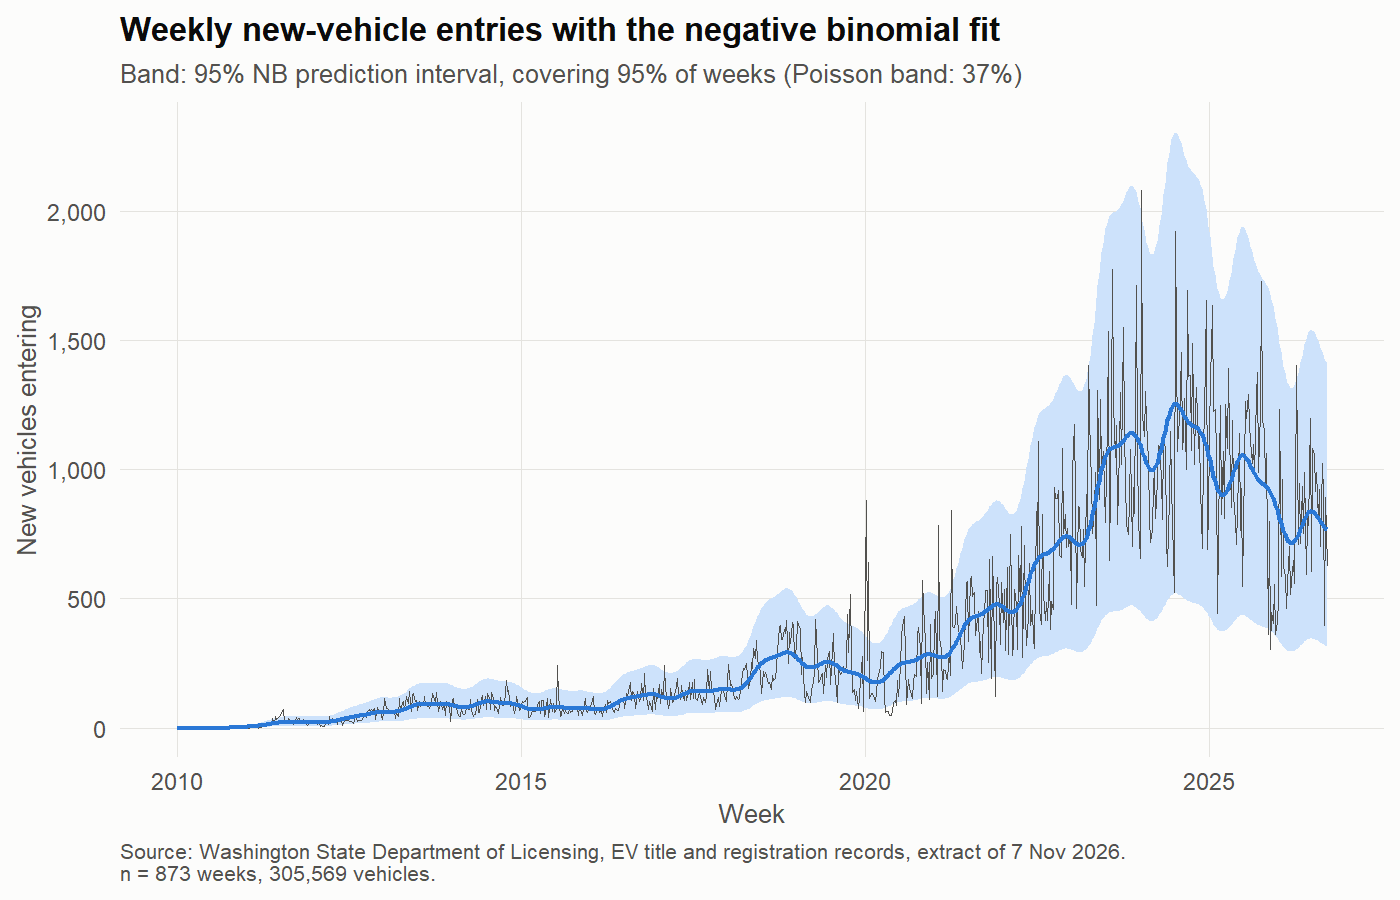
\includegraphics[width=6in,height=0.85\textheight,keepaspectratio]{12_01_weekly_entries_nb.png}
\caption{Weekly new-vehicle entries: Poisson and negative binomial fits (12\_01\_weekly\_entries\_nb.png)}
\end{figure}

\begin{itemize}
  \item \textbf{Discrete process:} weekly entries (873 weeks). Poisson is far too narrow (dispersion 9,627; its 95\% band covers 37\% of weeks). Negative binomial fits much better (AIC 9,571 vs 39,696; band covers 95\% of weeks); zero weeks observed 39, expected 38 (NB) and 45 (Poisson).
\end{itemize}

\begin{figure}[H]
\centering
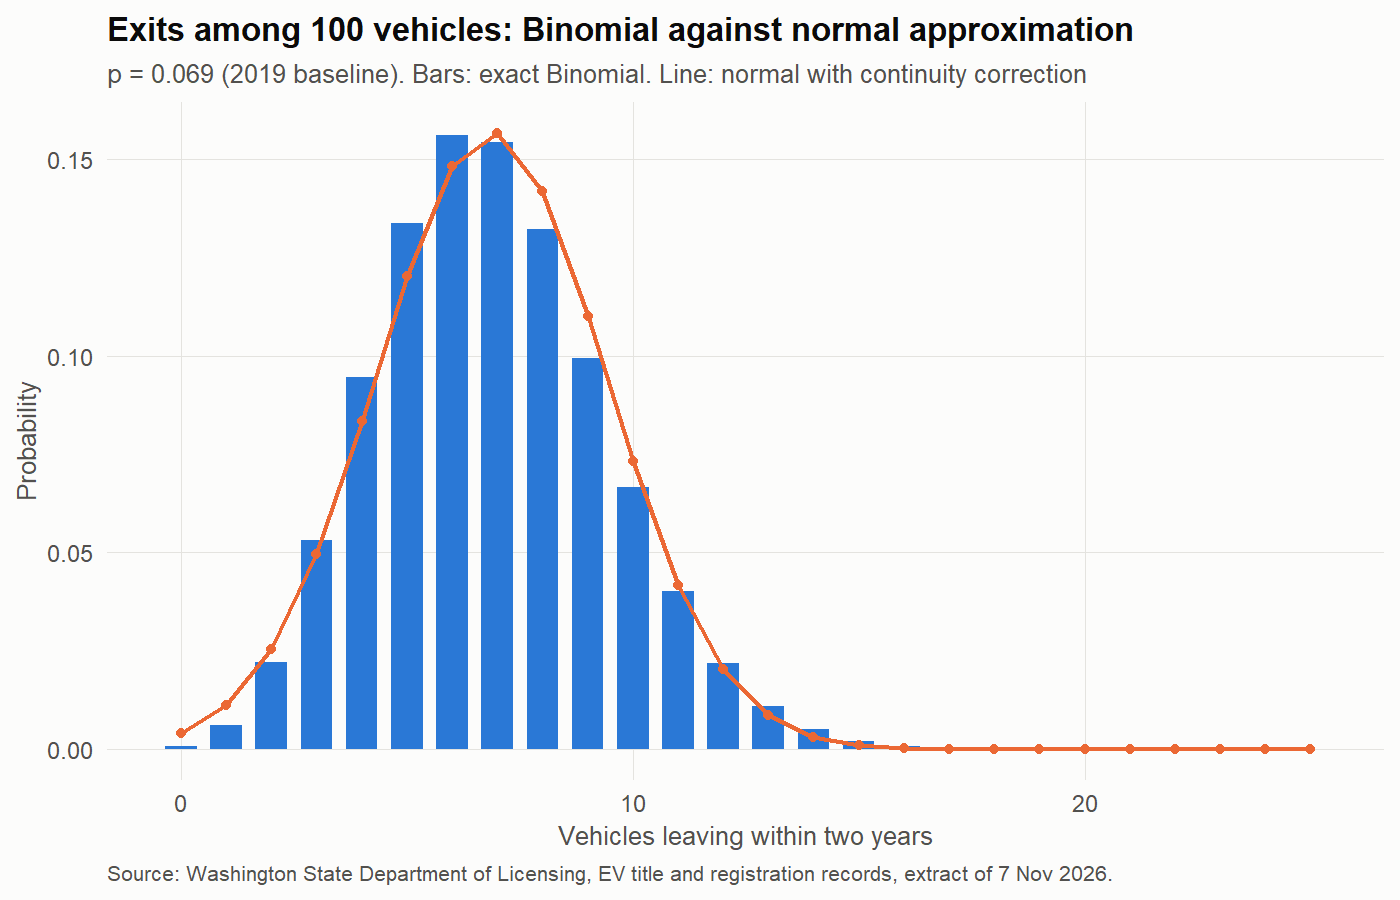
\includegraphics[width=6in,height=0.85\textheight,keepaspectratio]{12_02_binomial_vs_normal.png}
\caption{Binomial probabilities and the normal approximation (12\_02\_binomial\_vs\_normal.png)}
\end{figure}

\begin{itemize}
  \item \textbf{Binomial $\rightarrow$ normal:} model-year 2013 cohort active in 2021: 400 of 4,843 left (8.3\%) against 6.9\% expected from the 2019 two-year exit rate; exact P(X $\ge$ 400) = 0.0001. The normal approximation error falls as n grows (with continuity correction: $-0.083$ at n = 10, $-0.007$ at n = 1,000).
\end{itemize}

\begin{figure}[H]
\centering
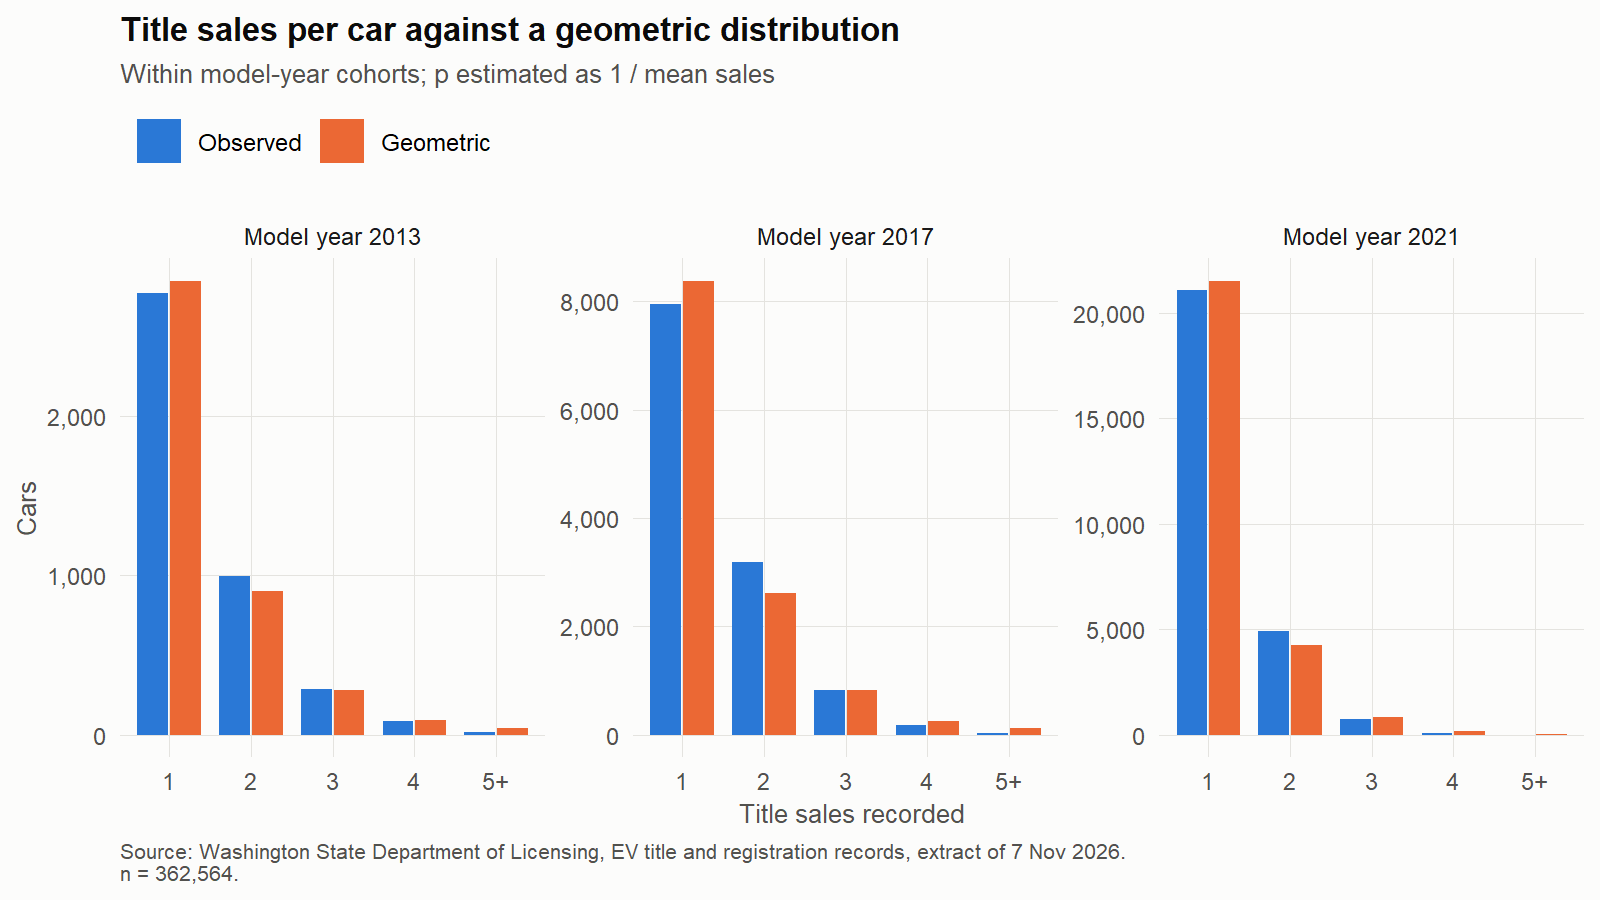
\includegraphics[width=6in,height=0.85\textheight,keepaspectratio]{12_03_geometric_sales.png}
\caption{Sale events per car against a geometric model (12\_03\_geometric\_sales.png)}
\end{figure}

\begin{itemize}
  \item \textbf{Geometric:} sales per car fit a geometric model overall ($\hat{p}$ = 0.85, goodness-of-fit p = 0.21) but not within single model years (p $<$ 0.001): the overall fit is a mixture of cohorts.
\end{itemize}

\begin{figure}[H]
\centering
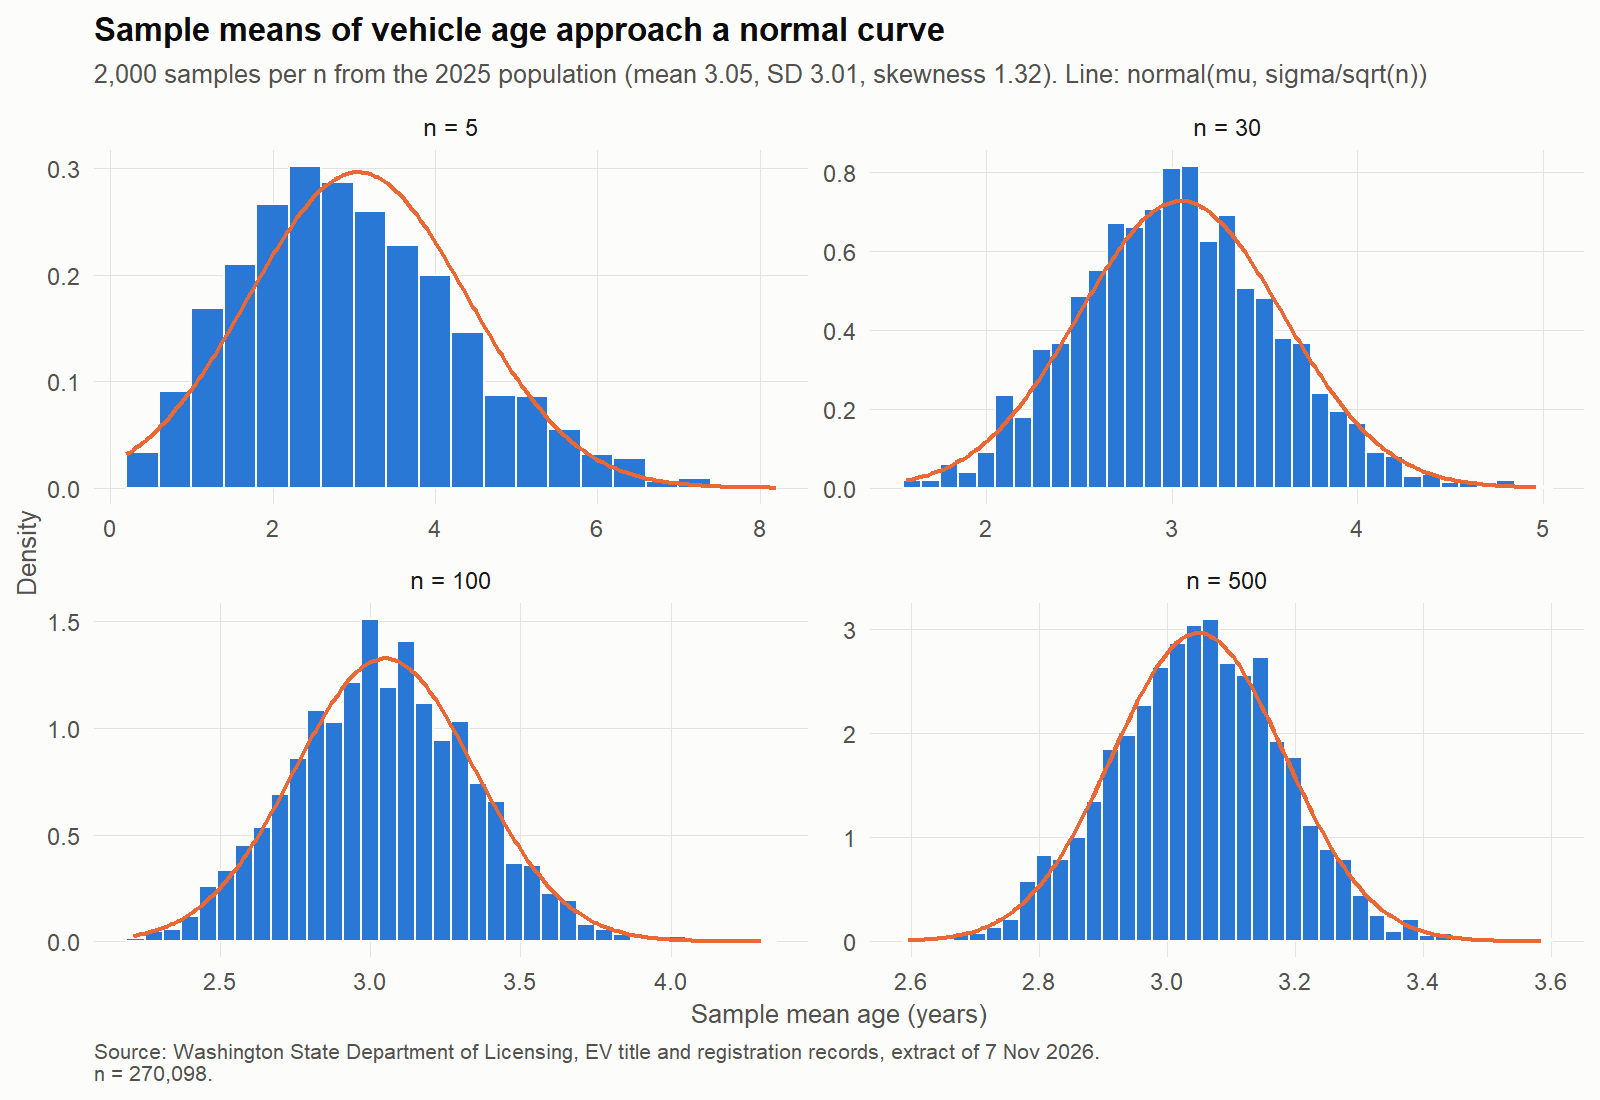
\includegraphics[width=6in,height=0.85\textheight,keepaspectratio]{12_04_clt_vehicle_age.png}
\caption{Sampling distribution of mean vehicle age (central limit theorem) (12\_04\_clt\_vehicle\_age.png)}
\end{figure}

\begin{itemize}
  \item \textbf{Sampling distribution of means:} vehicle age (skewness 1.32). SD of sample means matches $\sigma/\sqrt{n}$ (0.133 vs 0.135 at n = 500); skewness of the means falls from 0.51 (n = 5) to 0.02 (n = 500).
  \item \textbf{code: 12.1--12.4.}
\end{itemize}

\subsection{Hypothesis tests}

\begin{table}[htbp]
\centering
\footnotesize
\caption{Hypothesis tests (main, sensitivity and supporting) (13\_hypothesis\_tests.csv)}
\begin{tabularx}{\textwidth}{@{}XXrrrr@{}}
\toprule
\textbf{Test} & \textbf{Role} & \textbf{Estimate} & \textbf{95\% CI low} & \textbf{95\% CI high} & \textbf{p}\\
\midrule
Two-proportion z: King share 2025 vs 2019 & Main: spread & $-5.480$ & $-5.944$ & $-5.015$ & $<$ 0.001\\
Two-proportion z: King share 2025 vs 2019, gap-filled & Sensitivity & $-5.399$ & $-5.855$ & $-4.944$ & $<$ 0.001\\
Logistic LR test: PHEV vs BEV exit, adjusted for age, 2019 baseline & Sensitivity & 0.897 & 0.832 & 0.968 & 0.005\\
Logistic LR test: PHEV vs BEV exit, adjusted for age, 2021 baseline & Main: retention & 1.035 & 0.975 & 1.098 & 0.264\\
Logistic LR test: PHEV vs BEV exit, adjusted for age, 2023 baseline & Sensitivity & 0.967 & 0.924 & 1.012 & 0.143\\
One-sample z (mean): age of a 2025 sample vs 2019 mean & Supporting & 3.124 & 2.860 & 3.388 & $<$ 0.001\\
One-sample z (proportion): 2023 exit share vs 2019 rate & Supporting & 7.534 & 7.407 & 7.661 & $<$ 0.001\\
One-sample t: county log growth vs King's growth & Supporting & 1.806 & 1.720 & 1.891 & $<$ 0.001\\
One-sample t: as above, counties with 10+ vehicles in 2019 & Sensitivity & 1.795 & 1.718 & 1.873 & $<$ 0.001\\
Paired t: county BEV share 2025 vs 2019 & Supporting & 17.605 & 14.506 & 20.704 & $<$ 0.001\\
Welch t: age at last record, BEV vs PHEV & Supporting & $-0.829$ & $-0.892$ & $-0.766$ & $<$ 0.001\\
Welch t: age at the 2021 baseline, vehicles that left vs stayed & Supporting: feature separation & 0.215 & 0.142 & 0.288 & $<$ 0.001\\
Chi-square: exit by prior transfers (0, 1, 2+), 2021 baseline & Supporting: feature separation &  &  &  & $<$ 0.001\\
\bottomrule
\end{tabularx}
\end{table}

\begin{itemize}
  \item \textbf{Main spread test (H$_0$: King's share is the same in 2025 as in 2019):} two-proportion z = $-23.0$; share fell 5.5 points (95\% CI 5.0--5.9), p $\approx 3 \times 10^{-117}$. Reject H$_0$. Note: many vehicles are in both years, so the samples are not independent; the gap-filled count gives the same result.
  \item \textbf{Main retention test (H$_0$: after adjusting for age, BEVs and PHEVs are equally likely to leave within two years), 2021 baseline:} odds ratio 1.03 (0.97--1.10), likelihood-ratio p = 0.26. Don't reject H$_0$. Sensitivity: 0.90 (p = 0.005) at 2019, 0.97 (p = 0.14) at 2023.
  \item \textbf{One-sample z (mean):} mean age of a random 500-vehicle sample from 2025 = 3.12 vs the 2019 mean 2.58; z = 4.03, p $<$ 0.001 ($\sigma$ known from the 2025 records).
  \item \textbf{One-sample z (proportion):} 2023 exit share 7.53\% vs the 2019 rate; z = 10.9, p $<$ 0.001.
  \item \textbf{One-sample t:} mean county log growth 1.81 vs King's growth; t = 6.56, p $<$ 0.001 --- the average county grew faster than King.
  \item \textbf{Paired t:} county BEV share rose 17.6 points from 2019 to 2025 (14.5--20.7), t = 11.5, p $<$ 0.001, 35 counties (Wilcoxon p is in the table's effect\_size column).
  \item \textbf{Two-sample (Welch) t:} BEVs that left were 0.83 years younger at their last record than PHEVs that left (p $<$ 0.001).
  \item \textbf{Feature separation (2021 baseline):} vehicles that left were 0.21 years older (Welch p $<$ 0.001); exit differs by prior transfers (chi-square 84.8, df 2, p $<$ 0.001).
  \item \textbf{Interpret p-values with effect sizes:} with very large n, tiny differences are significant; the table's effect\_size column and the Bonferroni column help here.
  \item \textbf{code: 13.1--13.8.}
\end{itemize}

\subsection{Analysis of variance}

\begin{figure}[H]
\centering
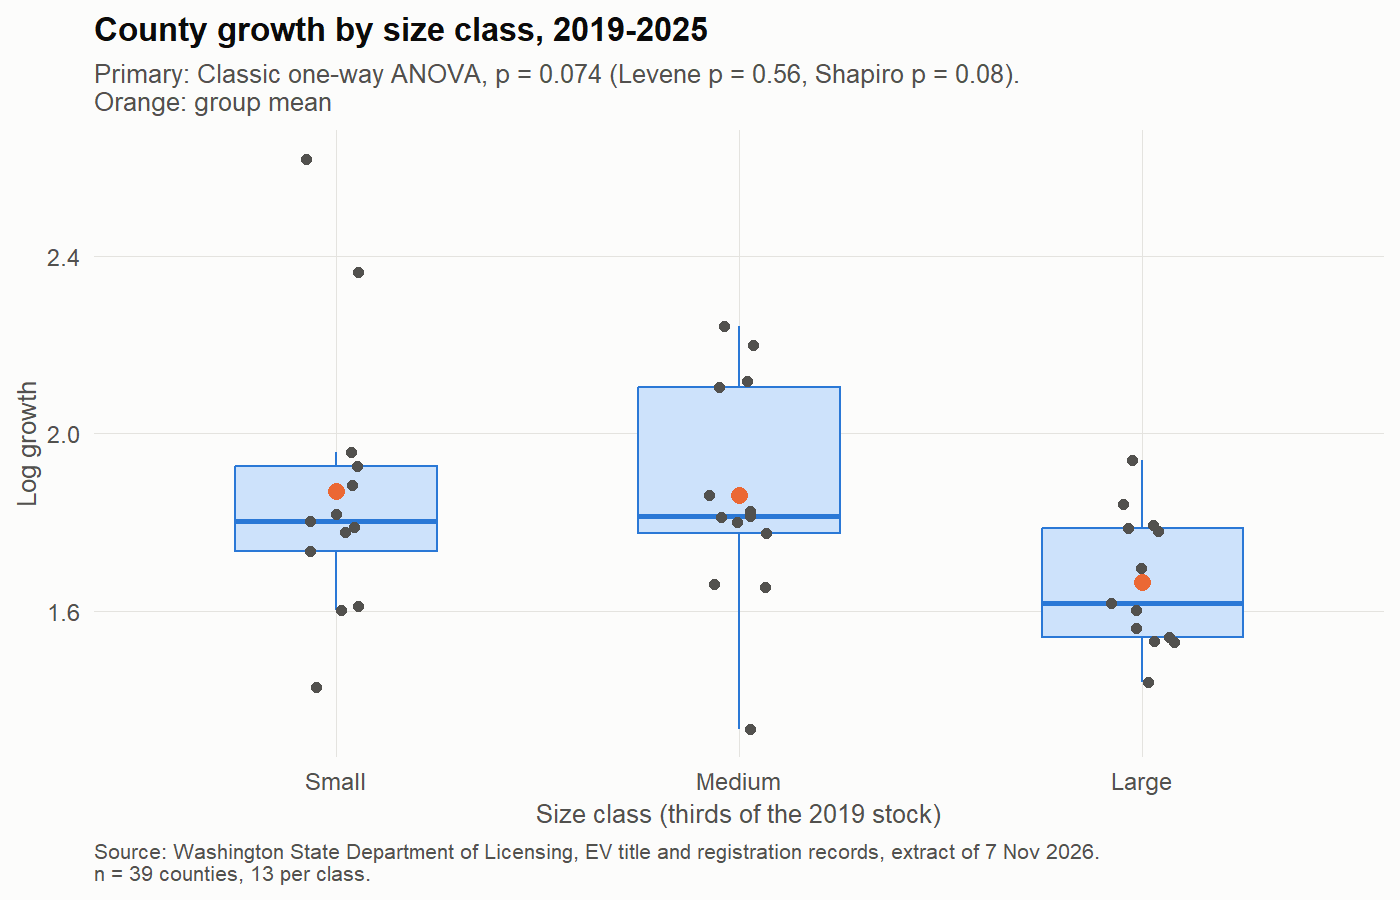
\includegraphics[width=6in,height=0.85\textheight,keepaspectratio]{13_01_anova_growth_by_size.png}
\caption{County growth 2019--2025 by size class (one-way ANOVA) (13\_01\_anova\_growth\_by\_size.png)}
\end{figure}

\begin{table}[htbp]
\centering
\small
\caption{One-way ANOVA: primary test and sensitivity checks (13\_anova\_oneway\_primary.csv)}
\begin{tabularx}{\textwidth}{@{}XrrrrX@{}}
\toprule
\textbf{Test} & \textbf{Statistic} & \textbf{df1} & \textbf{df2} & \textbf{p} & \textbf{Role}\\
\midrule
Classic one-way ANOVA & 2.80 & 2 & 36.0 & 0.074 & Primary (chosen by the assumption checks)\\
Welch ANOVA (unequal variances) & 4.05 & 2 & 21.8 & 0.032 & Sensitivity check\\
Kruskal-Wallis (no normality) & 6.22 & 2 &  & 0.045 & Sensitivity check\\
\bottomrule
\end{tabularx}
\end{table}

\begin{itemize}
  \item \textbf{One-way:} the primary test is chosen by the assumption checks, not the p-value: Levene p = 0.56 (equal variances) and Shapiro p = 0.075 (normal residuals), so classic ANOVA: F = 2.80, p = 0.074, $\eta^2$ = 0.13. Welch (0.032) and Kruskal--Wallis (0.045) are sensitivity checks; no Tukey pair is significant. Weak evidence that large counties grew less.
\end{itemize}

\begin{figure}[H]
\centering
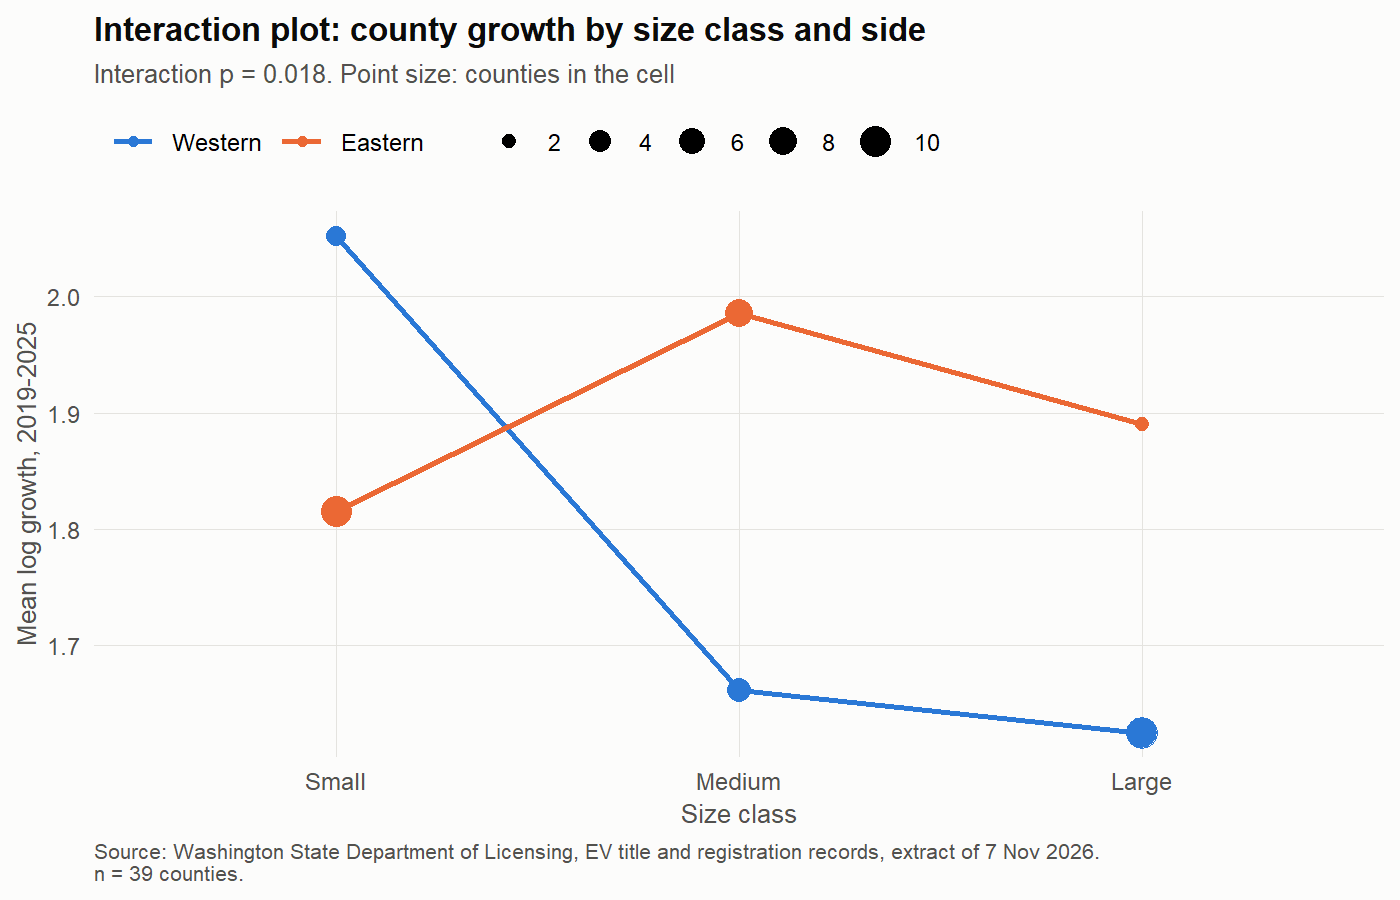
\includegraphics[width=6in,height=0.85\textheight,keepaspectratio]{13_02_anova_interaction.png}
\caption{Two-way ANOVA: size class by side of the Cascades (13\_02\_anova\_interaction.png)}
\end{figure}

\begin{itemize}
  \item \textbf{Two-way:} size class F = 3.45 (p = 0.044), side F = 2.29 (p = 0.14), interaction F = 4.57 (p = 0.018): the size effect differs between east and west. Cells are small; read with care.
\end{itemize}

\begin{figure}[H]
\centering
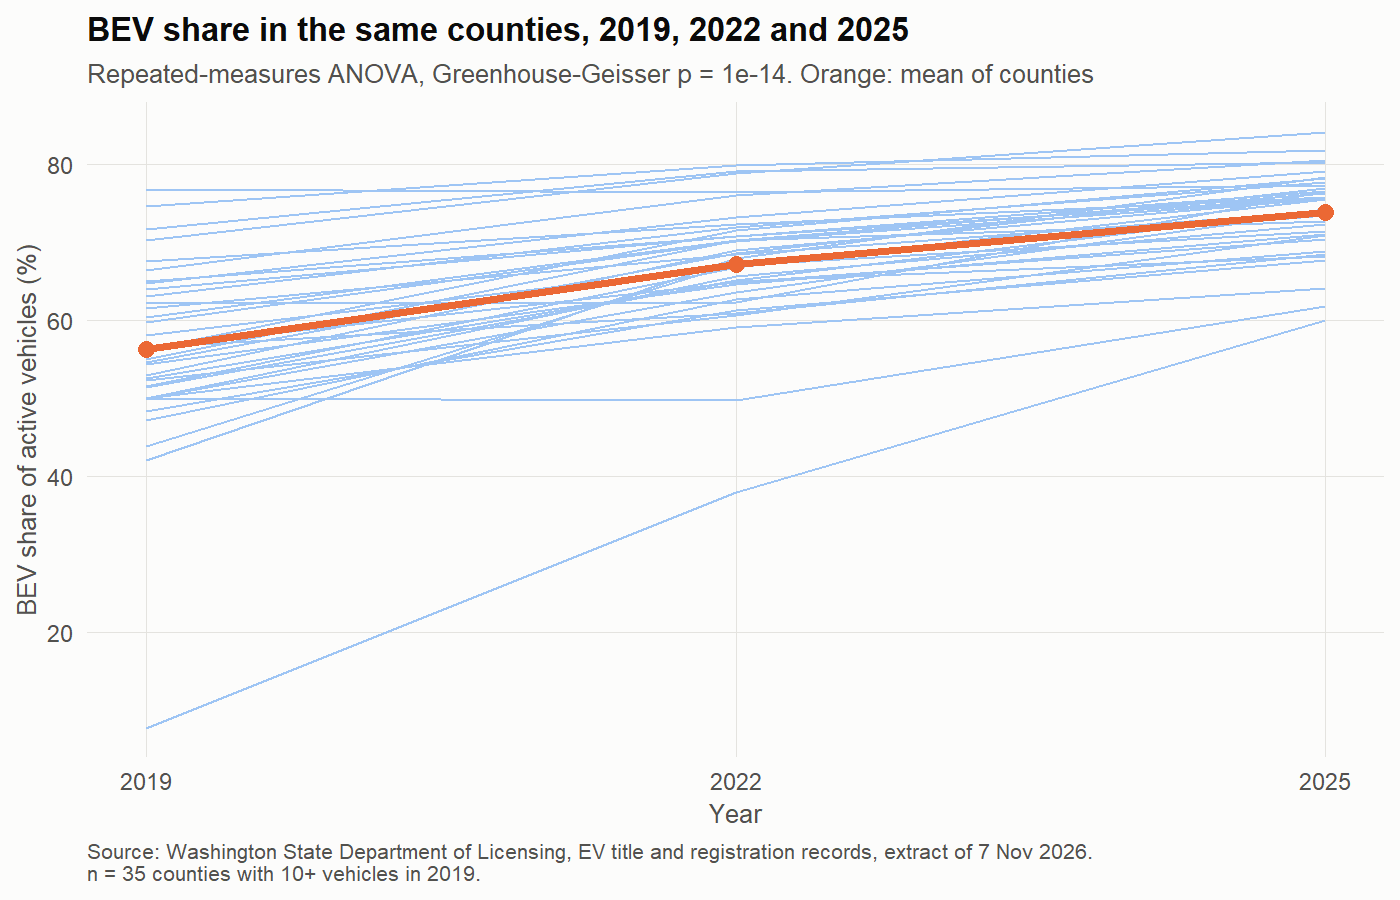
\includegraphics[width=6in,height=0.85\textheight,keepaspectratio]{13_03_rm_anova_bev_share.png}
\caption{BEV share in the same counties, 2019, 2022 and 2025 (13\_03\_rm\_anova\_bev\_share.png)}
\end{figure}

\begin{itemize}
  \item \textbf{Repeated measures:} mean county BEV share 56\% $\rightarrow$ 74\% (2019 $\rightarrow$ 2025). Mauchly's test rejects sphericity (p $<$ 0.001), so the Greenhouse--Geisser correction is used: p $\approx 10^{-14}$; partial $\eta^2$ = 0.78. Friedman test agrees.
\end{itemize}

\begin{figure}[H]
\centering
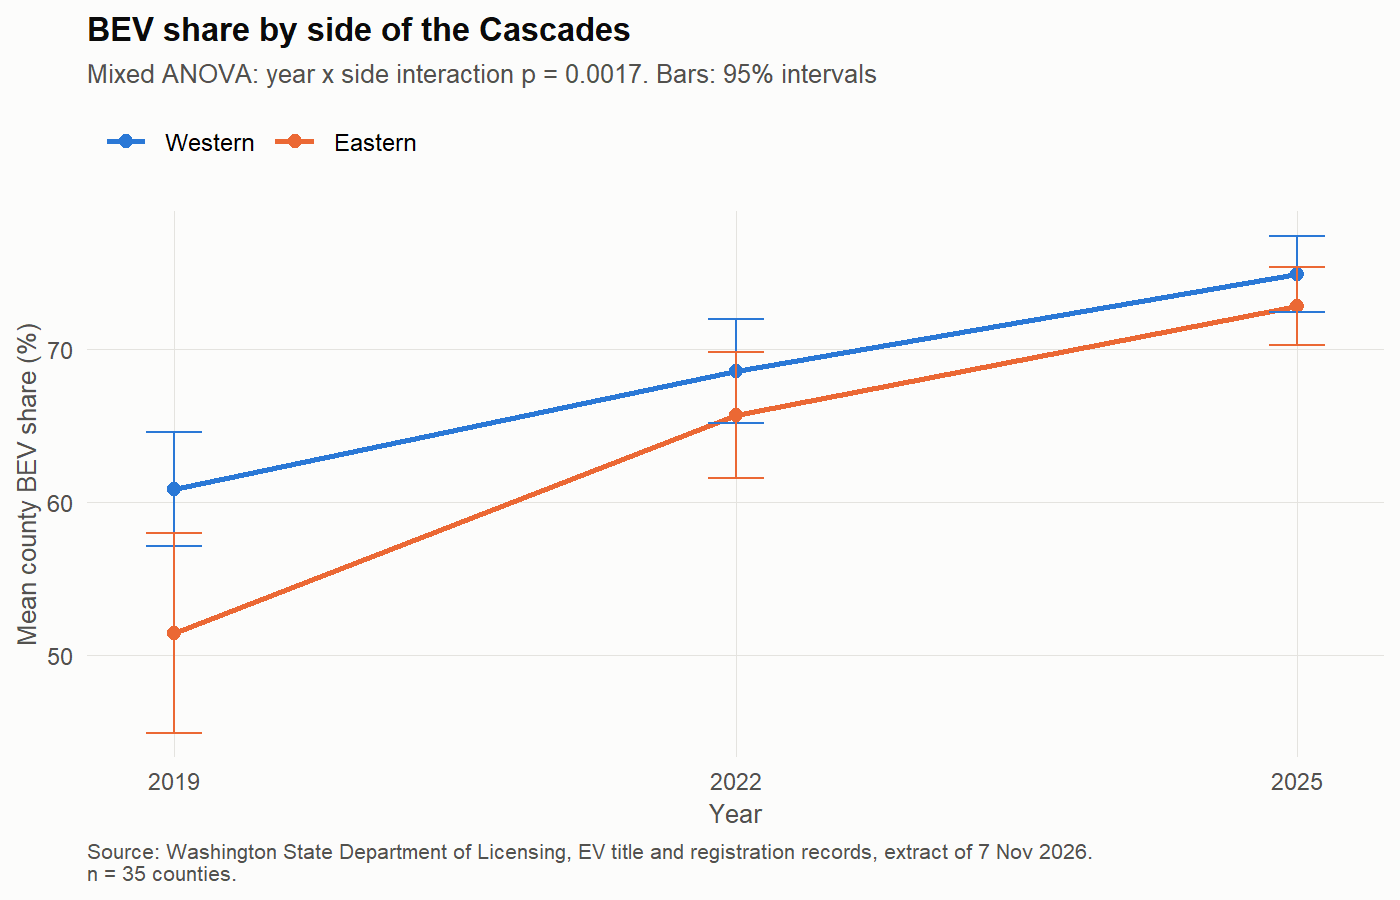
\includegraphics[width=6in,height=0.85\textheight,keepaspectratio]{13_04_mixed_anova_bev_share.png}
\caption{BEV share by side of the Cascades (mixed ANOVA) (13\_04\_mixed\_anova\_bev\_share.png)}
\end{figure}

\begin{itemize}
  \item \textbf{Mixed:} interaction side $\times$ year F = 7.02, p = 0.002: Eastern counties started lower (51\% vs 61\% in 2019) and caught up (73\% vs 75\% in 2025).
  \item \textbf{code: 13.9 (assumption helpers), 13.10--13.13.}
\end{itemize}

\subsection{Regression}

\begin{itemize}
  \item \textbf{Simple (39 counties):} log growth 2019--25 on log 2019 stock: slope $-0.038$ (95\% CI $-0.076$ to 0.001), p = 0.058, $R^2$ = 0.09. Smaller counties grew slightly faster; weak.
\end{itemize}

\begin{table}[htbp]
\centering
\small
\caption{Confidence and prediction intervals from the simple regression (14\_county\_intervals.csv)}
\begin{tabular}{rrrrrr}
\toprule
\textbf{2019 stock} & \textbf{Fitted log growth} & \textbf{CI low} & \textbf{CI high} & \textbf{PI low} & \textbf{PI high}\\
\midrule
10 & 1.90 & 1.77 & 2.04 & 1.38 & 2.43\\
100 & 1.82 & 1.73 & 1.90 & 1.30 & 2.33\\
1,000 & 1.73 & 1.62 & 1.84 & 1.21 & 2.25\\
10,000 & 1.64 & 1.46 & 1.82 & 1.10 & 2.18\\
\bottomrule
\end{tabular}
\end{table}

\begin{itemize}
  \item \textbf{Confidence vs prediction intervals:} the prediction interval is 3--6 times wider than the confidence interval: the average county is well estimated, a single county is not.
  \item \textbf{Multiple:} growth on log stock, used share and BEV share (2019): $R^2$ = 0.26 (adjusted 0.19), HC3 standard errors; used share +1.11 (p = 0.089); all VIF $\le$ 1.47 (no collinearity problem).
\end{itemize}

\begin{figure}[H]
\centering
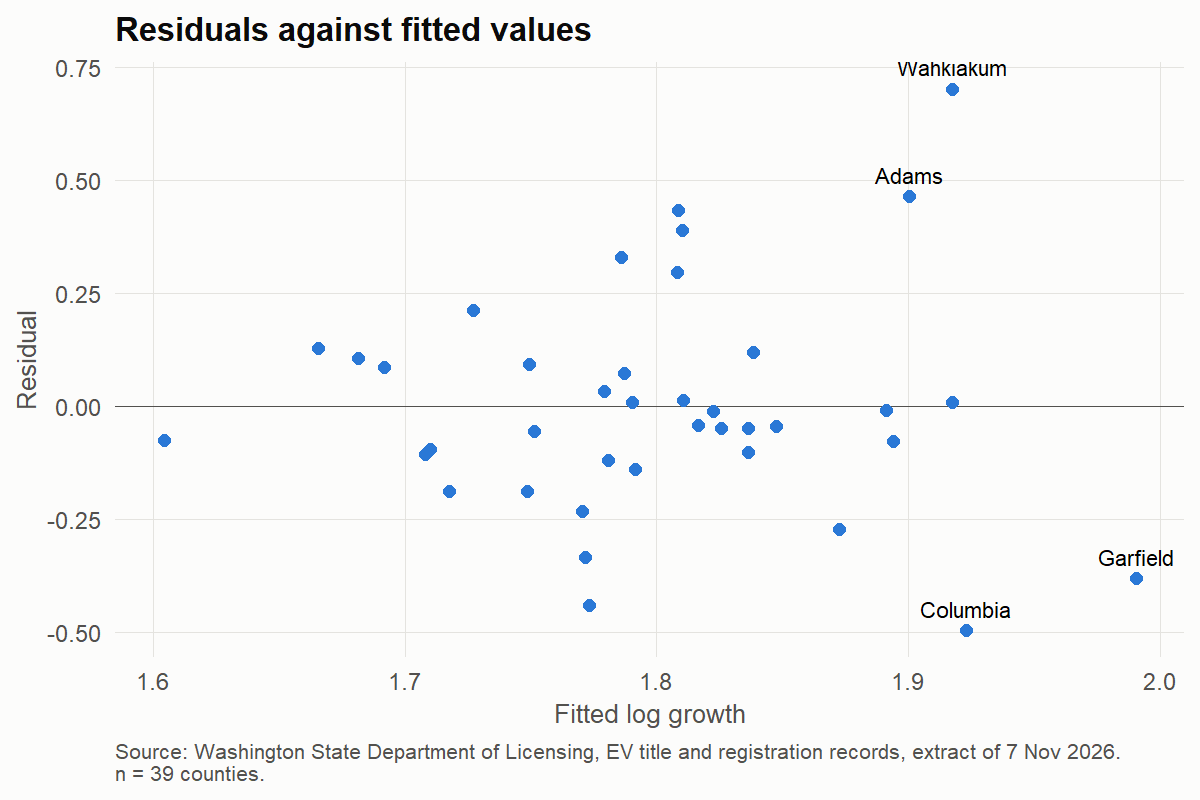
\includegraphics[width=6in,height=0.85\textheight,keepaspectratio]{14_01_county_residuals.png}
\caption{Residuals against fitted values, county regression (14\_01\_county\_residuals.png)}
\end{figure}

\begin{figure}[H]
\centering
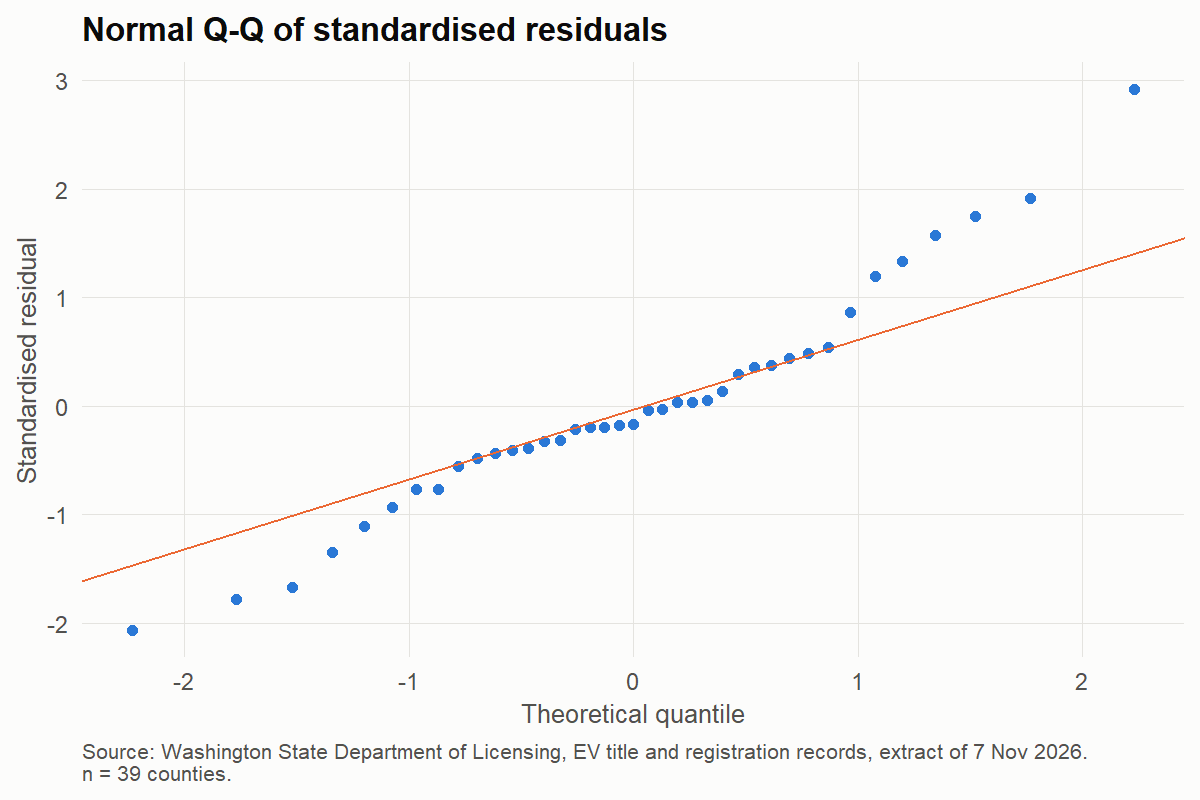
\includegraphics[width=6in,height=0.85\textheight,keepaspectratio]{14_02_county_qq.png}
\caption{Normal Q--Q plot of residuals (14\_02\_county\_qq.png)}
\end{figure}

\begin{figure}[H]
\centering
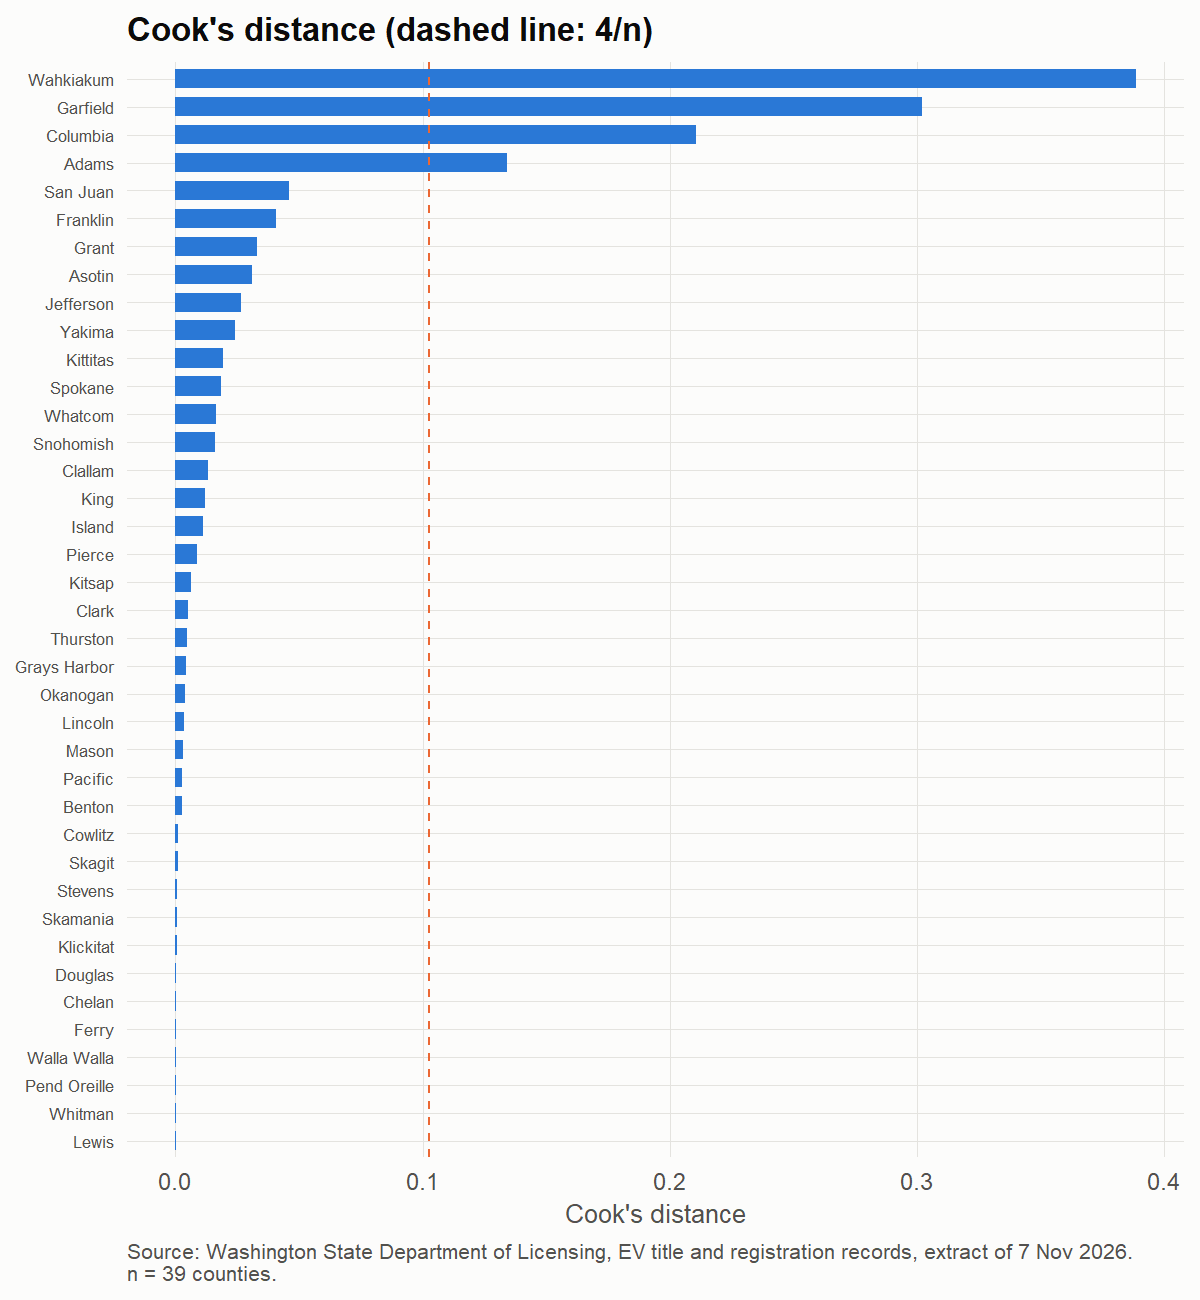
\includegraphics[width=6in,height=4.4in,keepaspectratio]{14_03_county_cooks.png}
\caption{Cook's distance (4/n rule) (14\_03\_county\_cooks.png)}
\end{figure}

\begin{itemize}
  \item \textbf{Specification model (used prices):} log real price on age, mileage, type and make: $R^2$ = 0.67 (141,153 sales); each year of age $-11.4\%$, each 10,000 miles $-4.7\%$, PHEV +8.1\% vs BEV (holding the rest fixed). Residuals: 14\_04\_spec\_residuals.png.
  \item \textbf{Logistic (exit within two years, trained at 2021, tested at 2023):} model A (base predictors) test AUC 0.522; model B (adds the vehicle's history) 0.569; DeLong p $\approx 10^{-76}$; McFadden $R^2$ 0.007 and 0.044. Both are weak: the reasons a vehicle leaves are not in the records.
\end{itemize}

\begin{table}[htbp]
\centering
\small
\caption{Logistic models: fit and discrimination (14\_logistic\_performance.csv)}
\begin{tabularx}{\textwidth}{@{}Xrrrrrr@{}}
\toprule
\textbf{Model} & \textbf{AIC} & \textbf{McFadden $R^2$} & \textbf{AUC train} & \textbf{AUC test} & \textbf{Brier (test)} & \textbf{Youden cut-off}\\
\midrule
A: base predictors & 44,987 & 0.007 & 0.563 & 0.522 & 0.070 & 0.075\\
B: plus history & 43,318 & 0.044 & 0.612 & 0.569 & 0.067 & 0.077\\
\bottomrule
\end{tabularx}
\end{table}

\begin{figure}[H]
\centering
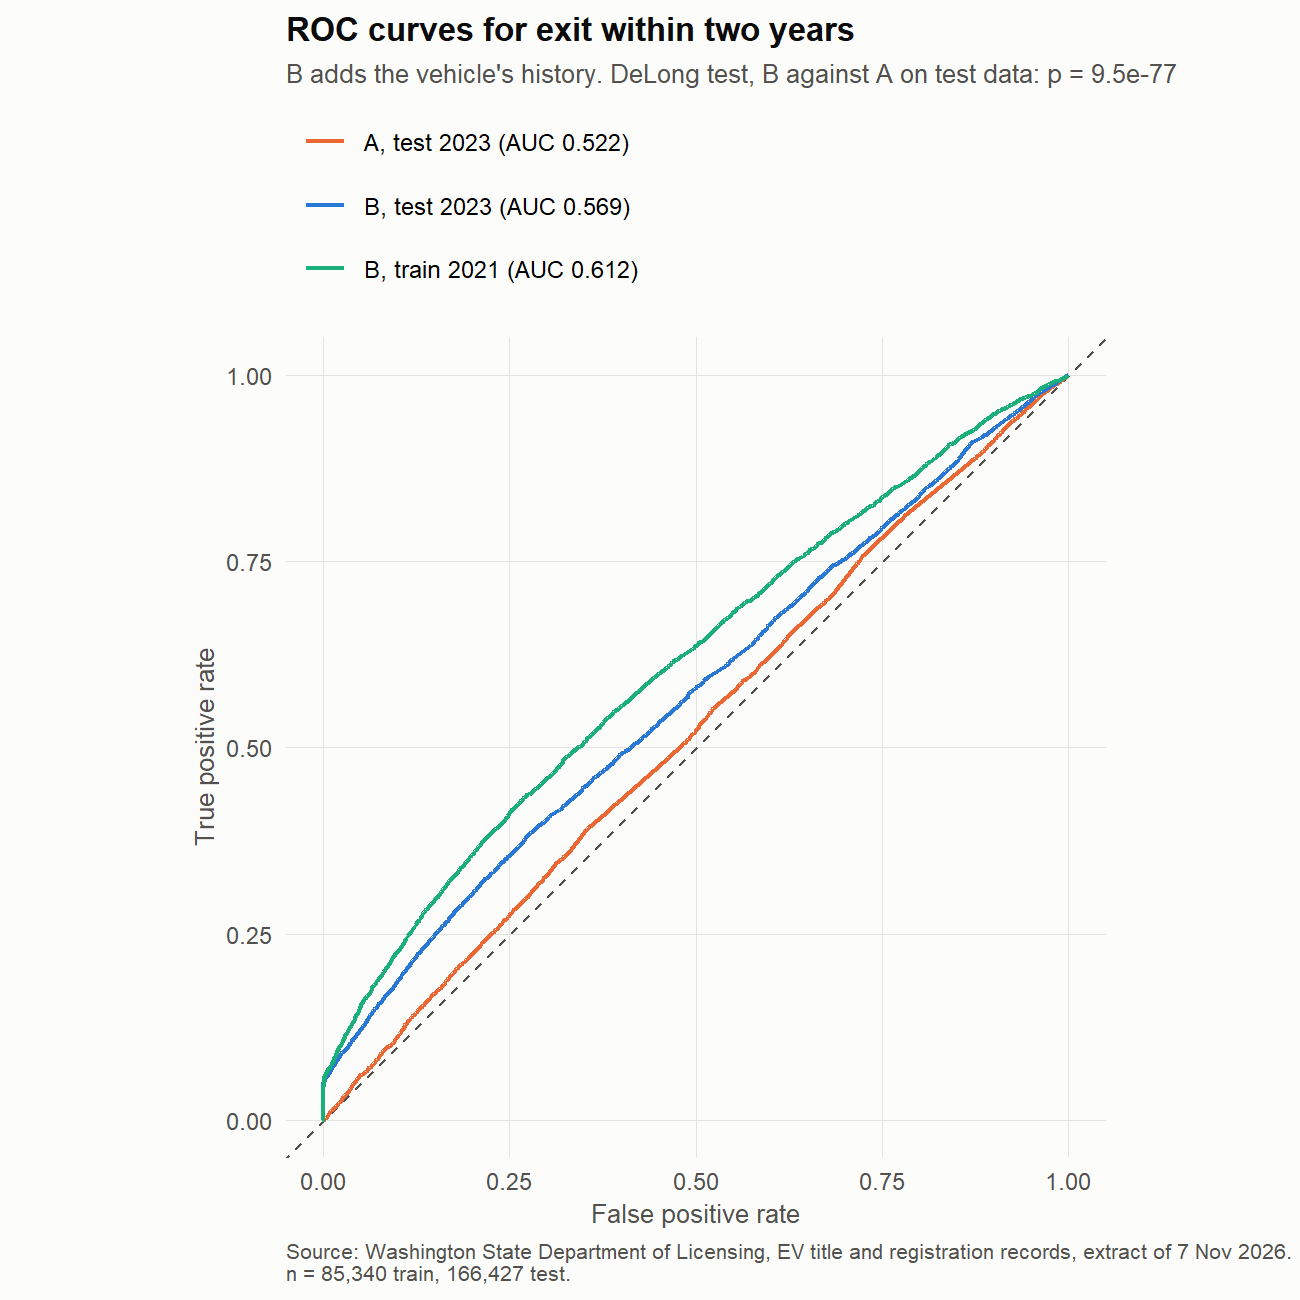
\includegraphics[width=6in,height=0.85\textheight,keepaspectratio]{14_06_logistic_roc.png}
\caption{ROC curves on the 2023 test data (14\_06\_logistic\_roc.png)}
\end{figure}

\begin{figure}[H]
\centering
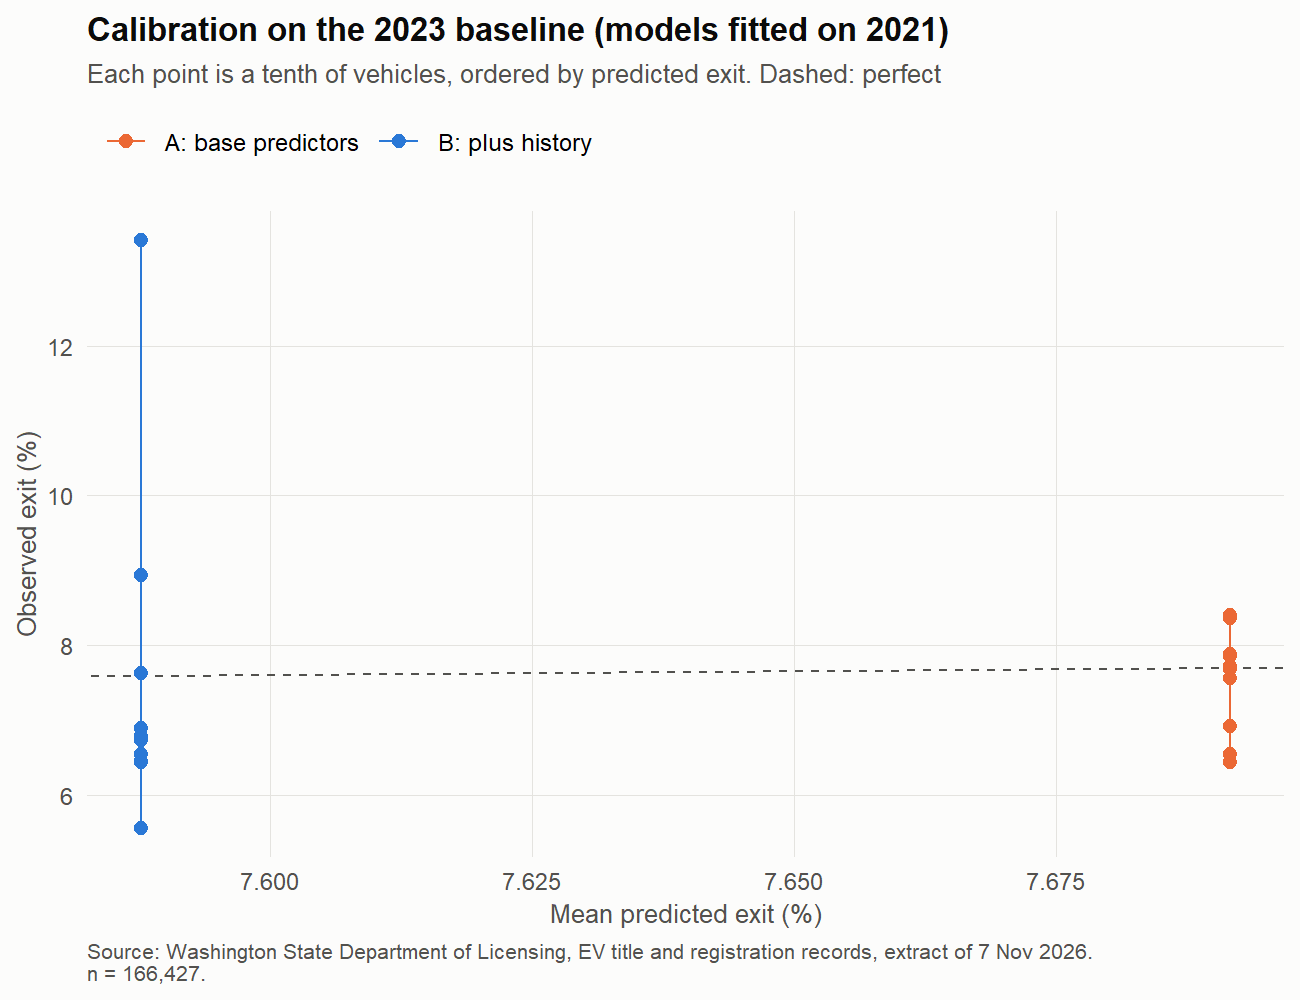
\includegraphics[width=6in,height=0.85\textheight,keepaspectratio]{14_05_logistic_calibration.png}
\caption{Calibration on the 2023 test data: predicted against observed exit, by tenth (14\_05\_logistic\_calibration.png)}
\end{figure}

\begin{itemize}
  \item \textbf{Calibration:} both models get the overall rate right (mean predicted 7.7\% and 7.6\% vs 7.5\% observed). Model B's tenths run from 5.6\% to 13.4\% observed exit and follow the diagonal in the middle, but over-predict the top tenth (15.5\% predicted vs 13.4\%). Model A's observed rates only span 6.4--8.4\%, and its top tenth predicts 12.3\% against 8.4\% observed: little separation. Table: 14\_logistic\_calibration.csv.
\end{itemize}

\begin{figure}[H]
\centering
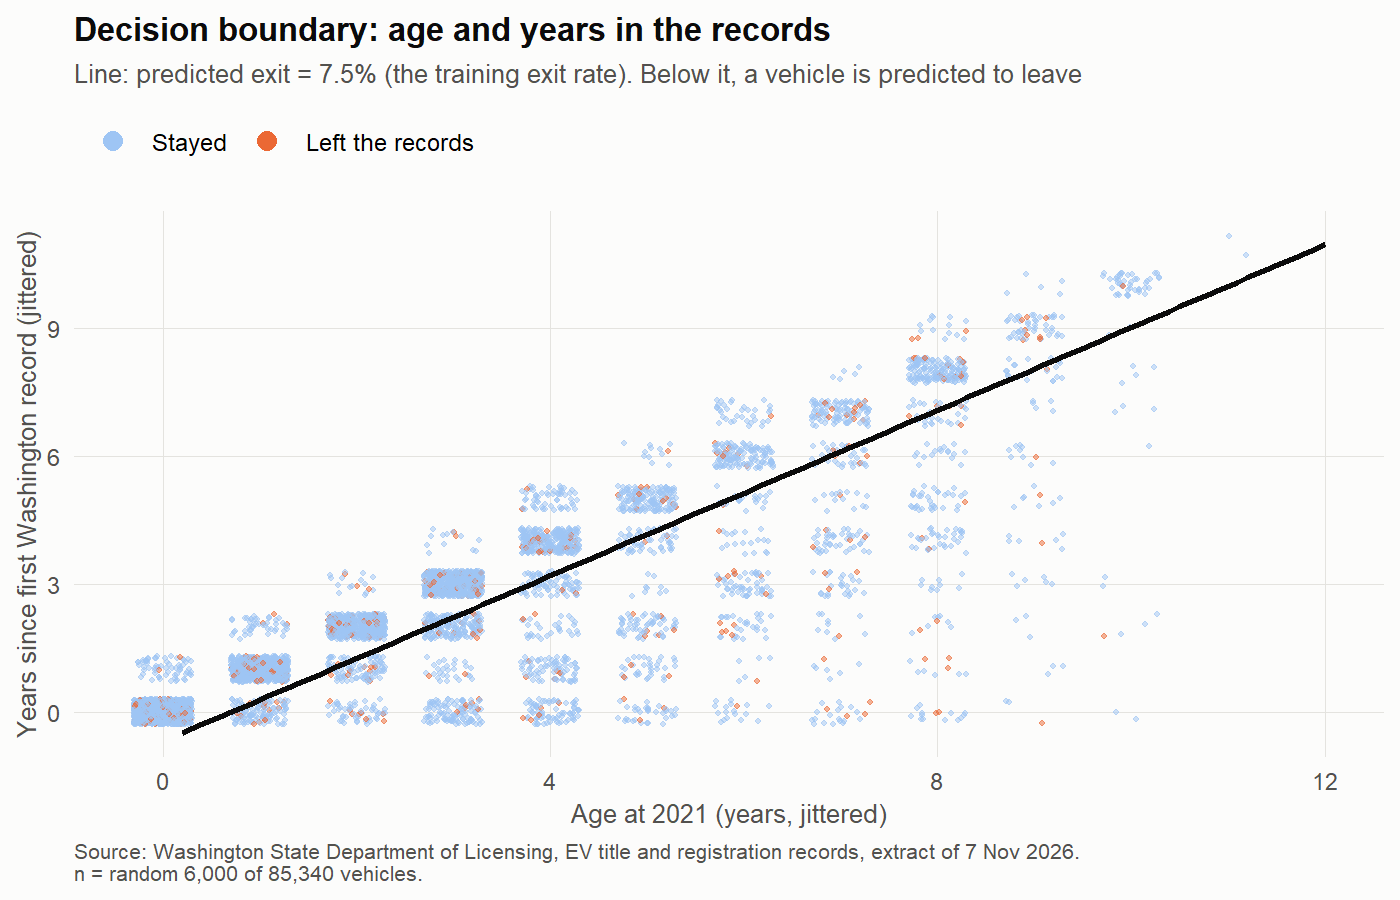
\includegraphics[width=6in,height=0.85\textheight,keepaspectratio]{14_07_decision_boundary.png}
\caption{Decision boundary on age and years in the records (14\_07\_decision\_boundary.png)}
\end{figure}

\begin{figure}[H]
\centering
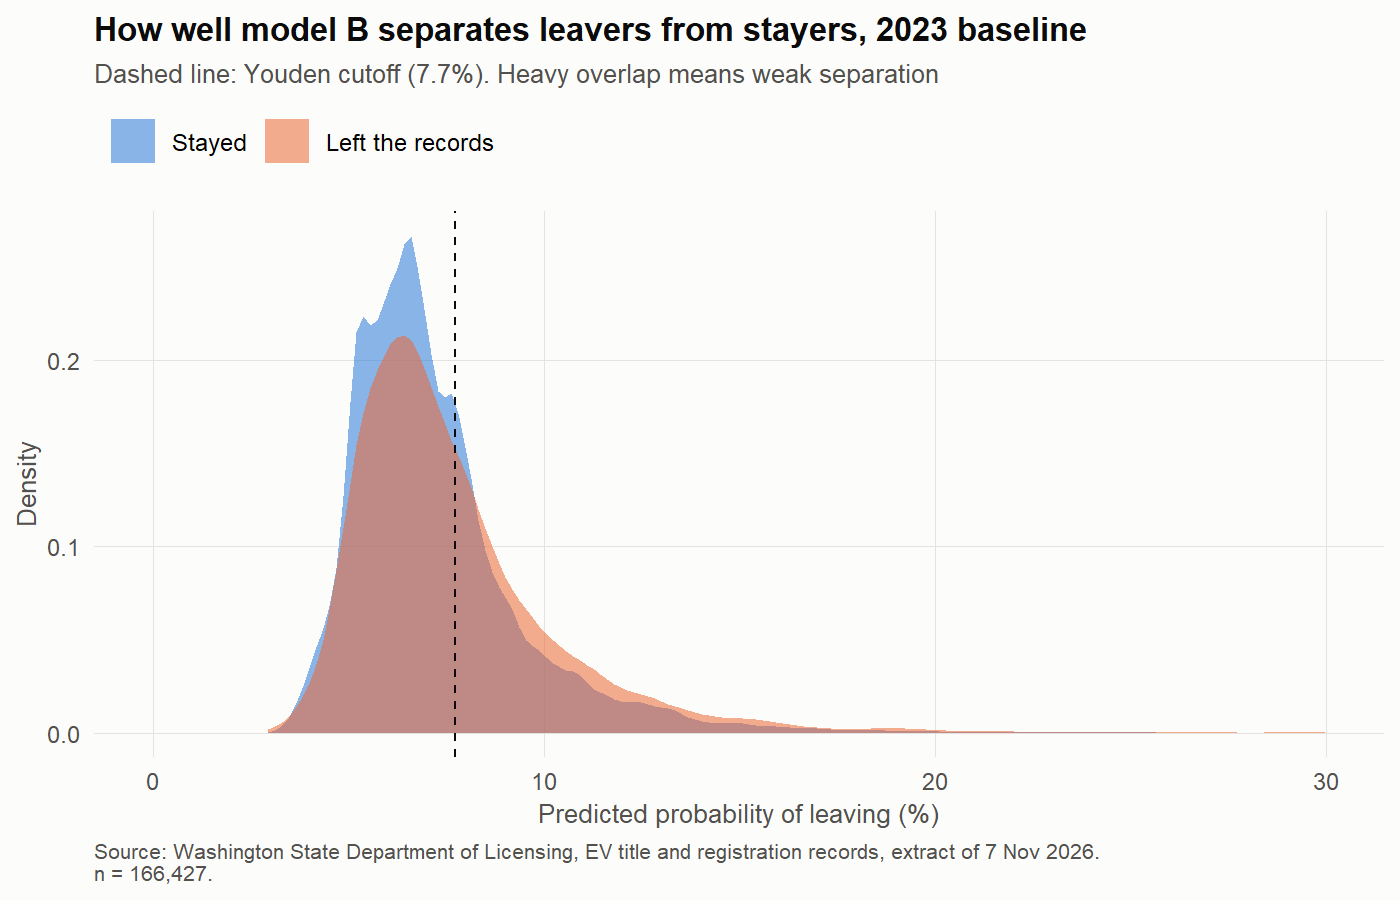
\includegraphics[width=6in,height=0.85\textheight,keepaspectratio]{14_08_logistic_class_separation.png}
\caption{Predicted probabilities for vehicles that left and stayed (14\_08\_logistic\_class\_separation.png)}
\end{figure}

\begin{itemize}
  \item \textbf{Odds and adjusted probabilities (model A, 2021 training data):} adjusted two-year exit 6.9\% in King vs about 8\% elsewhere; 7.1\% with no prior transfer vs 10.8\% with two or more; 15.2\% for truck/commercial use vs 7.4\% passenger; PHEV 6.5\% vs BEV 7.9\% with make held fixed (this differs from the age-only main test because it compares within makes). Table: 14\_logistic\_adjusted\_probabilities.csv; odds ratios: 14\_logistic\_odds\_ratios.csv.
  \item \textbf{Cut-off and confusion matrix:} at 0.5 almost nothing is predicted to leave (exit rate 7.5\%); at the Youden cut-off model B has sensitivity 0.40 and specificity 0.70 (14\_logistic\_confusion\_test.csv).
  \item \textbf{Linearity of the logit (Box--Tidwell):} age passes (p = 0.79), so it enters as a straight-line term (rule fixed before fitting). Tenure shows curvature (p $<$ 0.001); it is used only in the two-predictor decision boundary (14.9), so mention it as a limit there (14\_logistic\_linearity.csv).
  \item \textbf{code: 14.1--14.2 (county), 14.3 (specification), 14.4--14.9 (logistic).}
\end{itemize}

\subsection{Extensions beyond the brief}

\begin{figure}[H]
\centering
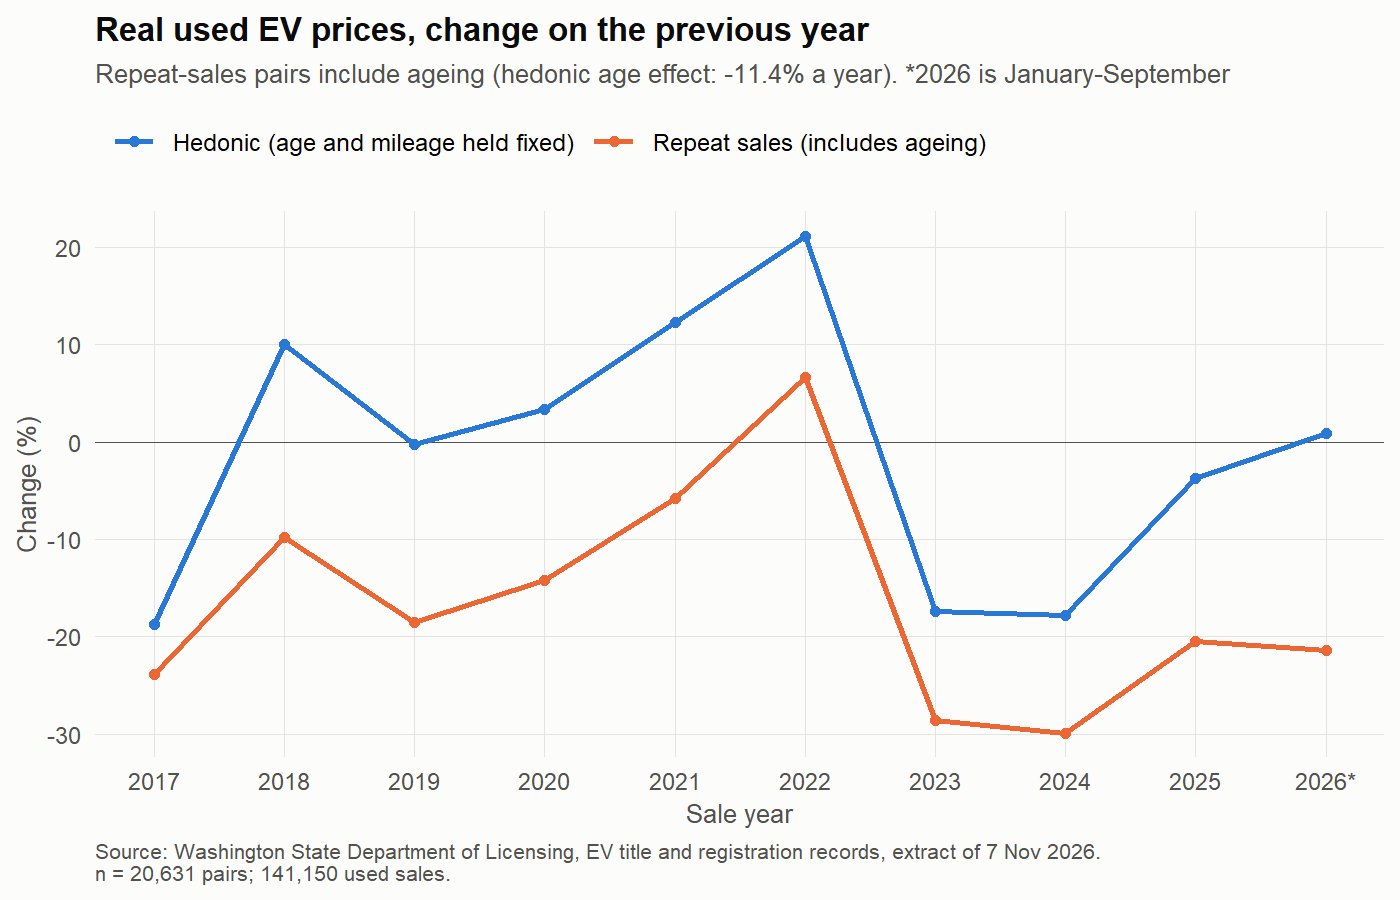
\includegraphics[width=6in,height=0.85\textheight,keepaspectratio]{15_01_used_price_index.png}
\caption{Real used EV prices, change on the previous year (15\_01\_used\_price\_index.png)}
\end{figure}

\begin{itemize}
  \item \textbf{Used prices (ext. 1):} 20,631 repeat-sale pairs on 17,088 cars. The repeat-sales index includes ageing; the hedonic index holds age and mileage fixed: +21\% in 2022, about $-17\%$ in each of 2023 and 2024. Each year of age $\approx -11.4\%$ in real price. code: 15.1--15.7.
\end{itemize}

\begin{figure}[H]
\centering
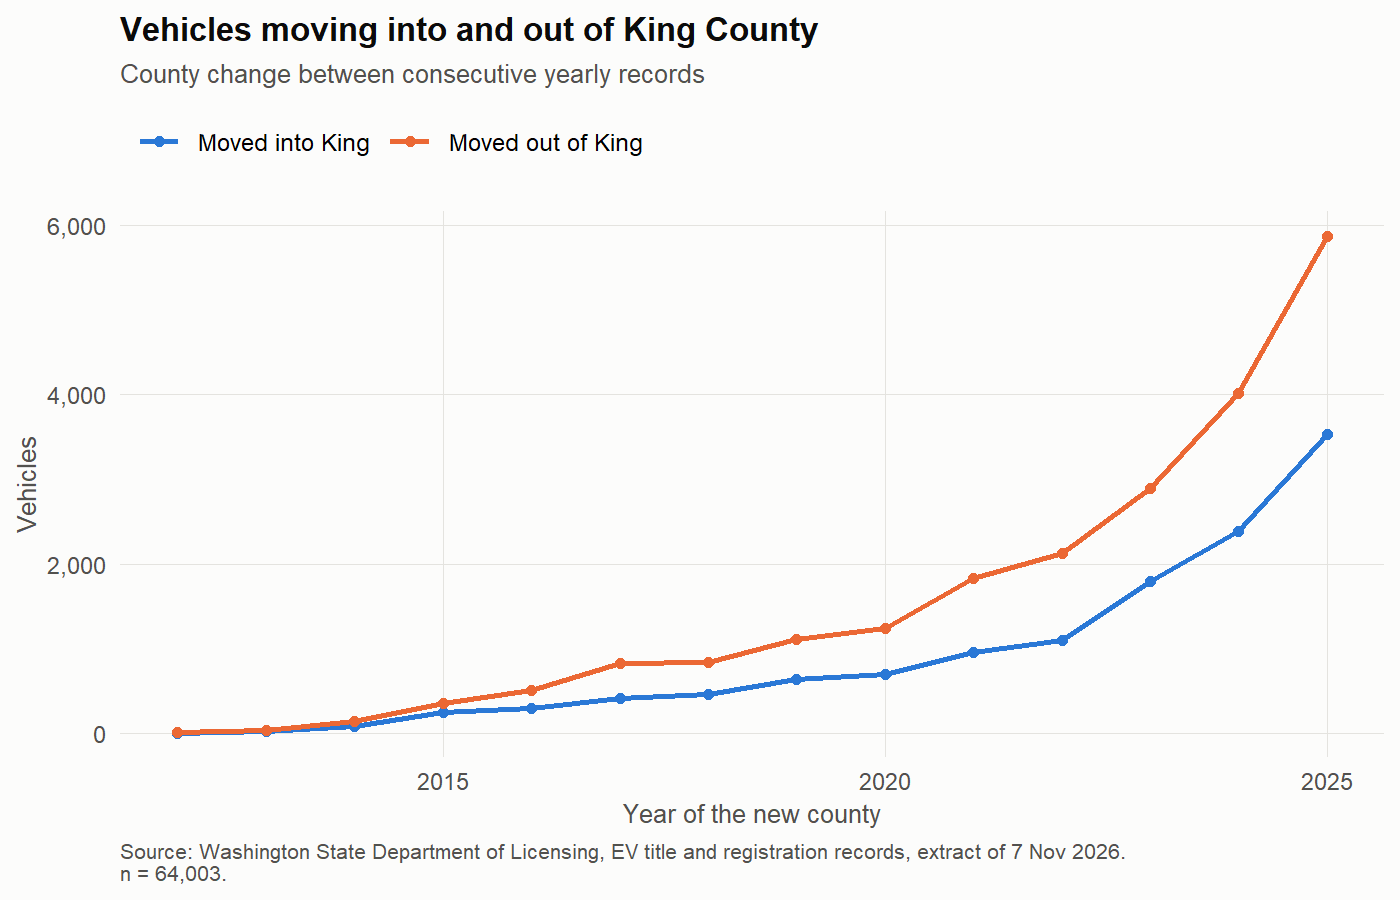
\includegraphics[width=6in,height=0.85\textheight,keepaspectratio]{16_01_king_moves.png}
\caption{Vehicles moving into and out of King County (16\_01\_king\_moves.png)}
\end{figure}

\begin{itemize}
  \item \textbf{Movement (ext. 3):} in a year with a title transfer, 37.1\% of King vehicles left the county, against 2.1\% without one. code: section 16.
\end{itemize}

\begin{figure}[H]
\centering
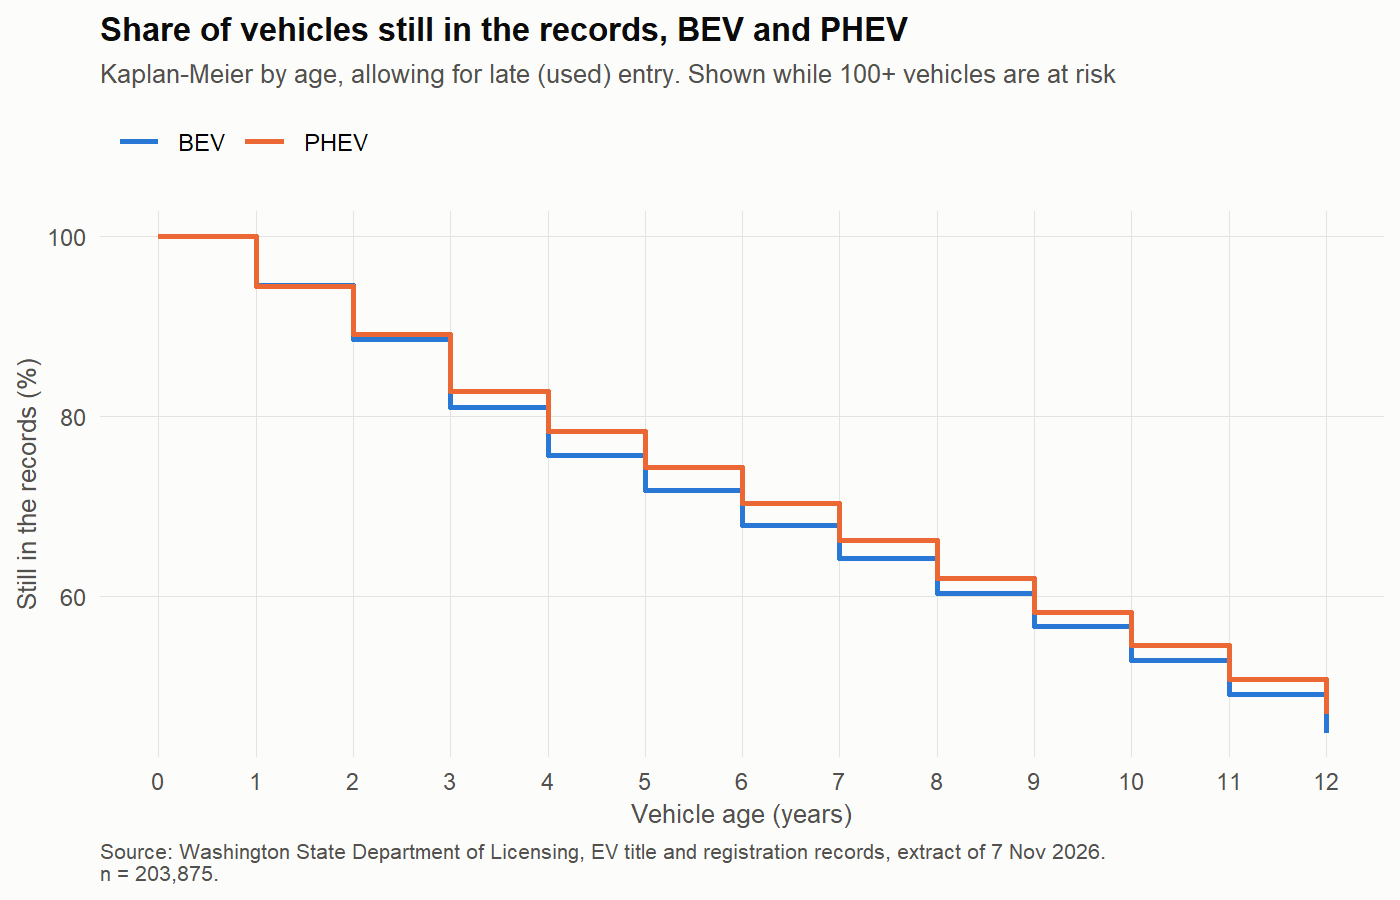
\includegraphics[width=6in,height=0.85\textheight,keepaspectratio]{17_01_survival_by_type.png}
\caption{Share of vehicles still in the records by age, BEV and PHEV (17\_01\_survival\_by\_type.png)}
\end{figure}

\begin{itemize}
  \item \textbf{Survival (ext. 4):} at age 5, 72\% of BEVs and 74\% of PHEVs are still in the records; at age 10, 53\% and 55\%. Cox hazard ratio for PHEV 0.92 over 2010--2023, but only before 2020: by period it is 0.69--0.79 up to 2019 and 1.03 for 2021--2023; proportional-hazards check p = 0.024. So the main conclusion (no difference in the current fleet) holds. code: 17, 17.1.
  \item \textbf{Electric range (ext. 5):} no evidence that range is associated with leaving (odds ratio 0.94 per 100 miles, p = 0.38; BEVs of model year 2020 or earlier). code: section 18.
\end{itemize}

\begin{figure}[H]
\centering
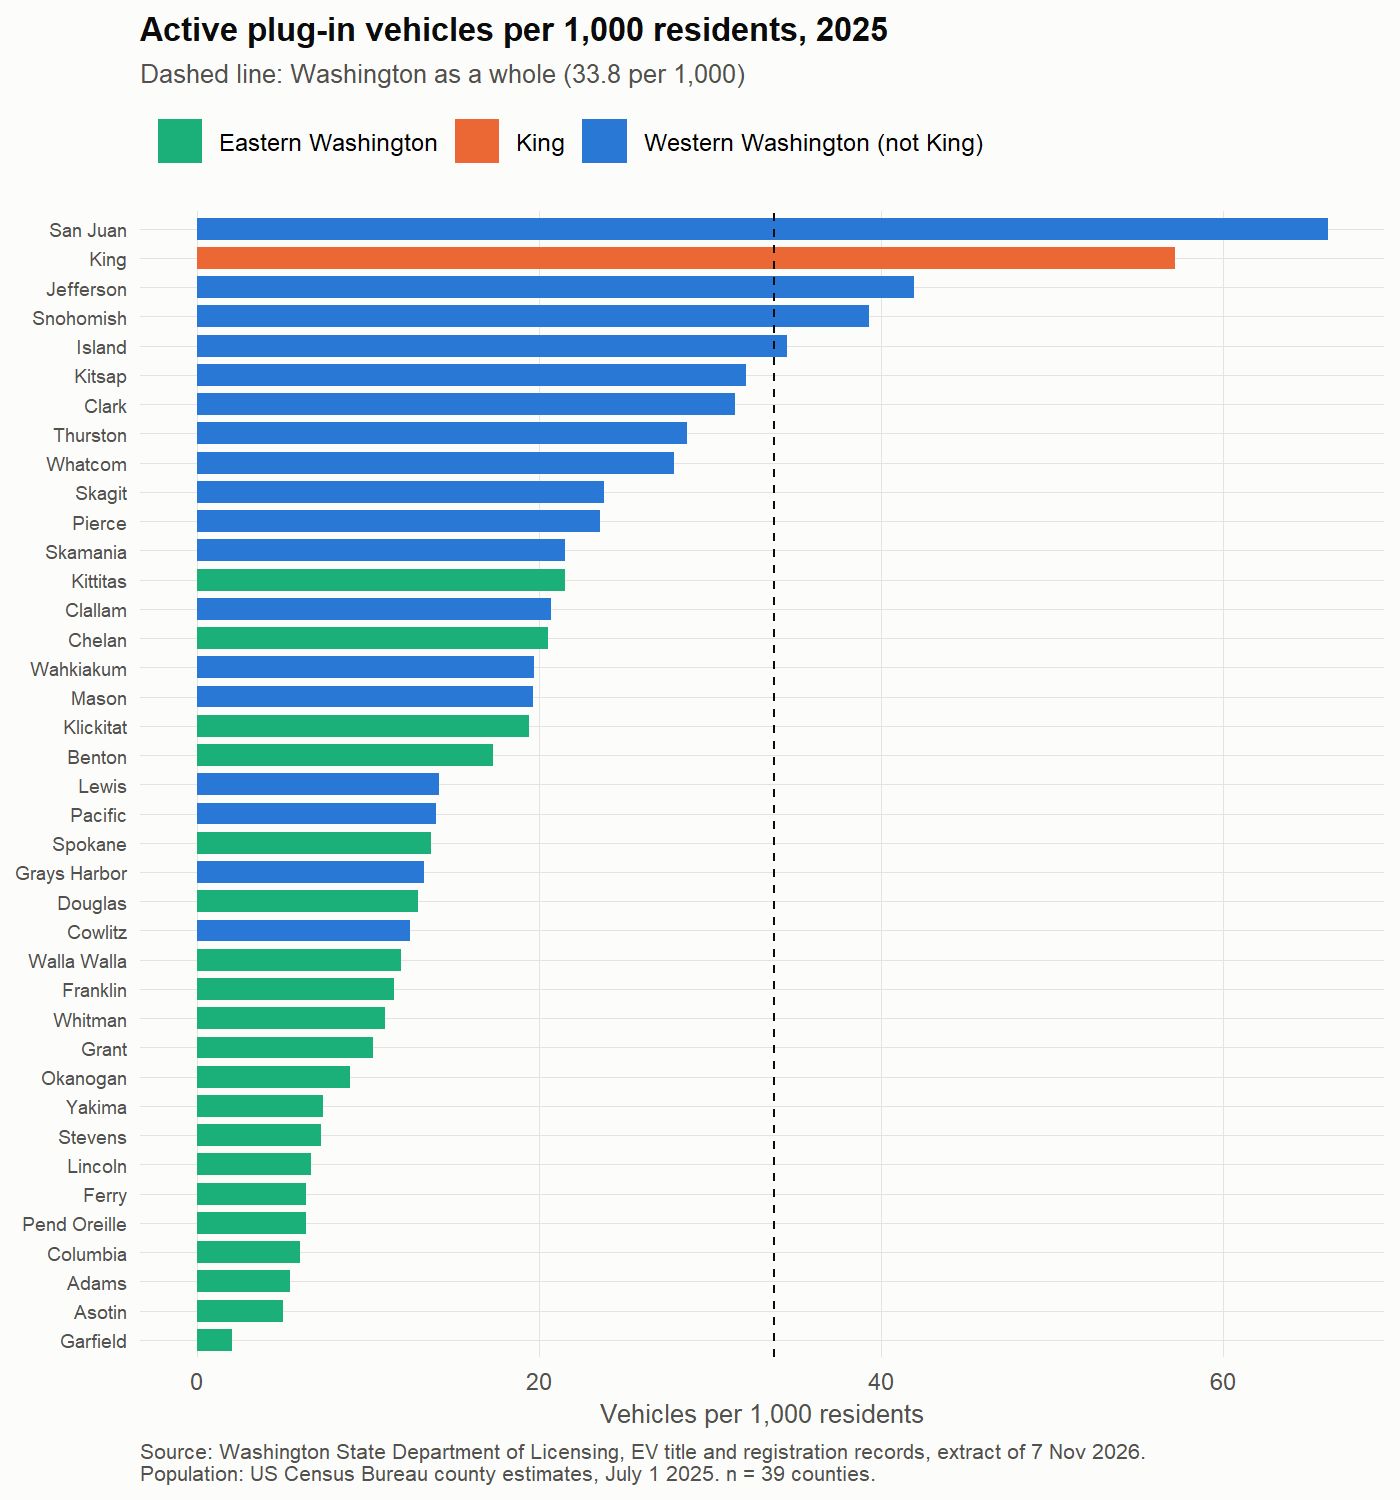
\includegraphics[width=6in,height=0.85\textheight,keepaspectratio]{19_01_ev_per_1000_2025.png}
\caption{Plug-in vehicles per 1,000 residents by county, 2025 (19\_01\_ev\_per\_1000\_2025.png)}
\end{figure}

\begin{figure}[H]
\centering
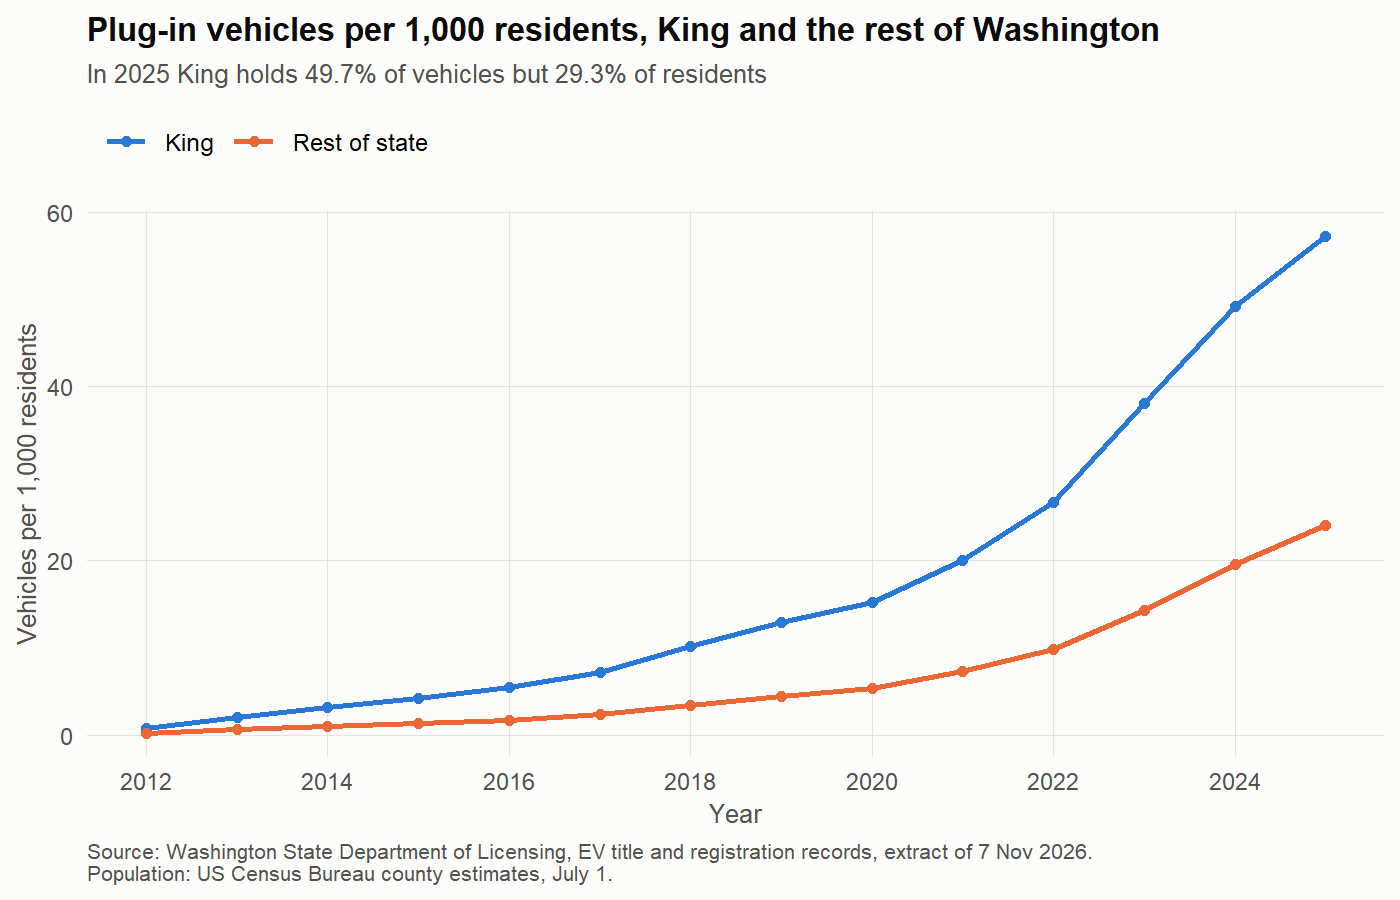
\includegraphics[width=6in,height=0.85\textheight,keepaspectratio]{19_02_ev_per_1000_king_vs_rest.png}
\caption{Vehicles per 1,000 residents, King and the rest of the state (19\_02\_ev\_per\_1000\_king\_vs\_rest.png)}
\end{figure}

\begin{itemize}
  \item \textbf{Per resident (ext. 2):} 33.8 per 1,000 in the state, 57.2 in King, 24.0 elsewhere (2025). San Juan County is highest (66.2). King has 49.7\% of vehicles and 29.3\% of residents. code: 19.
\end{itemize}

\begin{figure}[H]
\centering
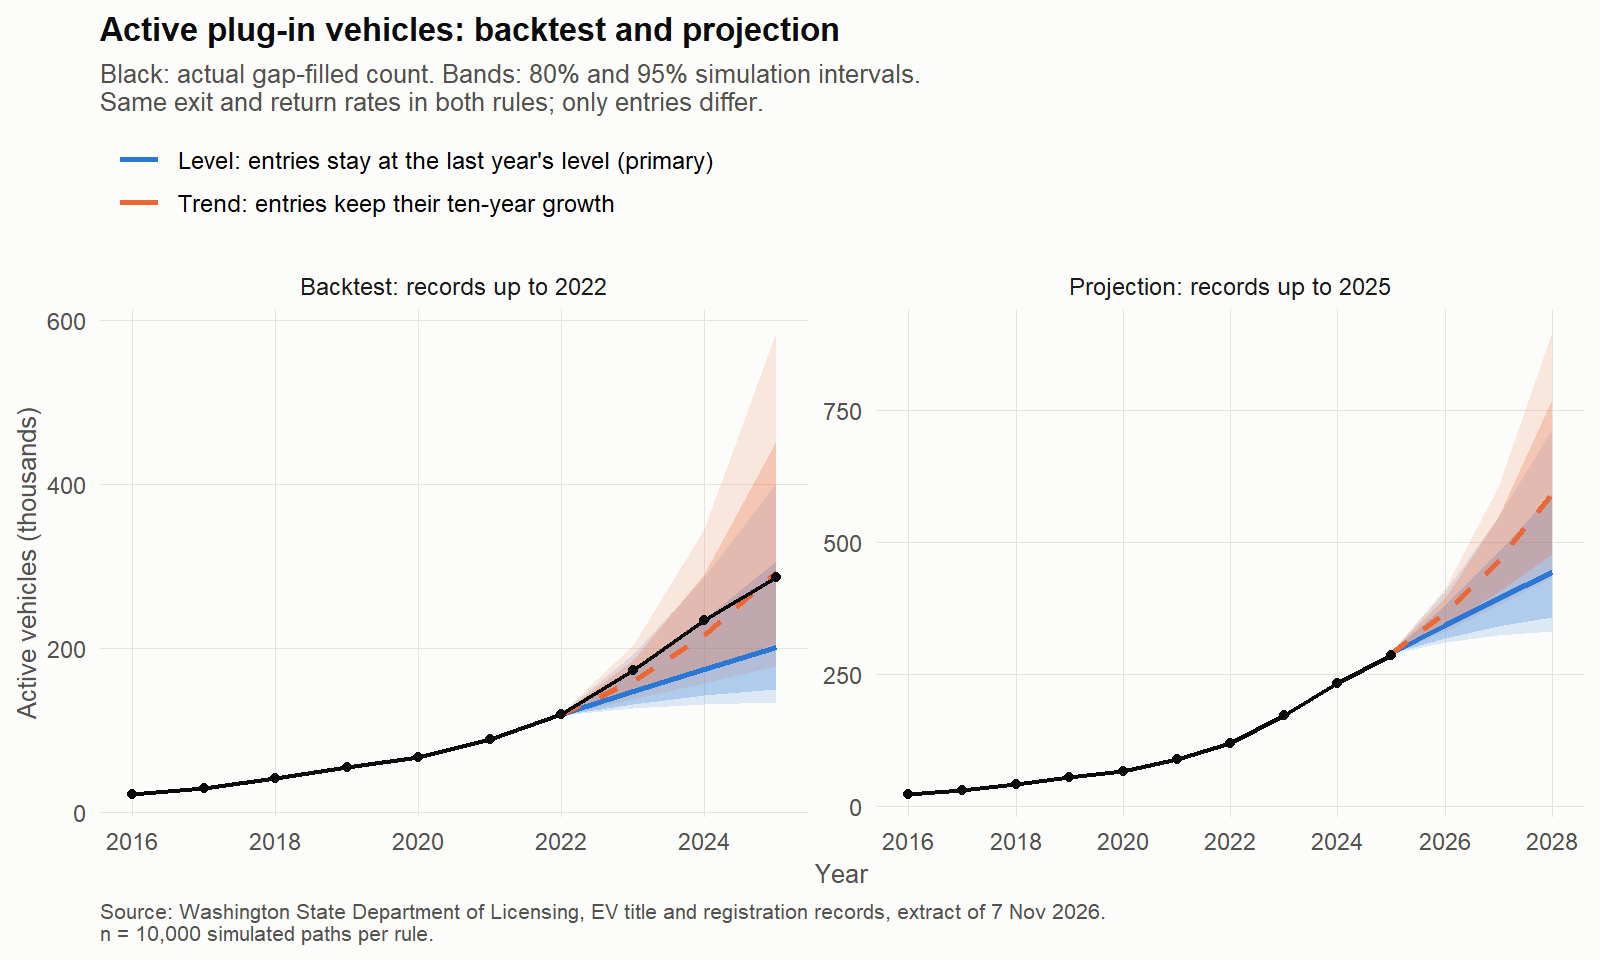
\includegraphics[width=6in,height=0.85\textheight,keepaspectratio]{20_01_projection.png}
\caption{Projected active vehicles to 2028, with 80\% and 95\% intervals (20\_01\_projection.png)}
\end{figure}

\begin{itemize}
  \item \textbf{Projection (ext. 6):} about 444,000 active vehicles in 2028 (95\% interval 331,000--714,000); high scenario about 593,000. Backtest from 2022: within 1\% with actual entries, 30\% low with projected entries (entries jumped in 2023), yet inside the 80\% interval. January--September 2026 entries are 11.8\% below 2025. Limits: rates held constant; one backtest origin. code: 20.1--20.4.
\end{itemize}

\begin{figure}[H]
\centering
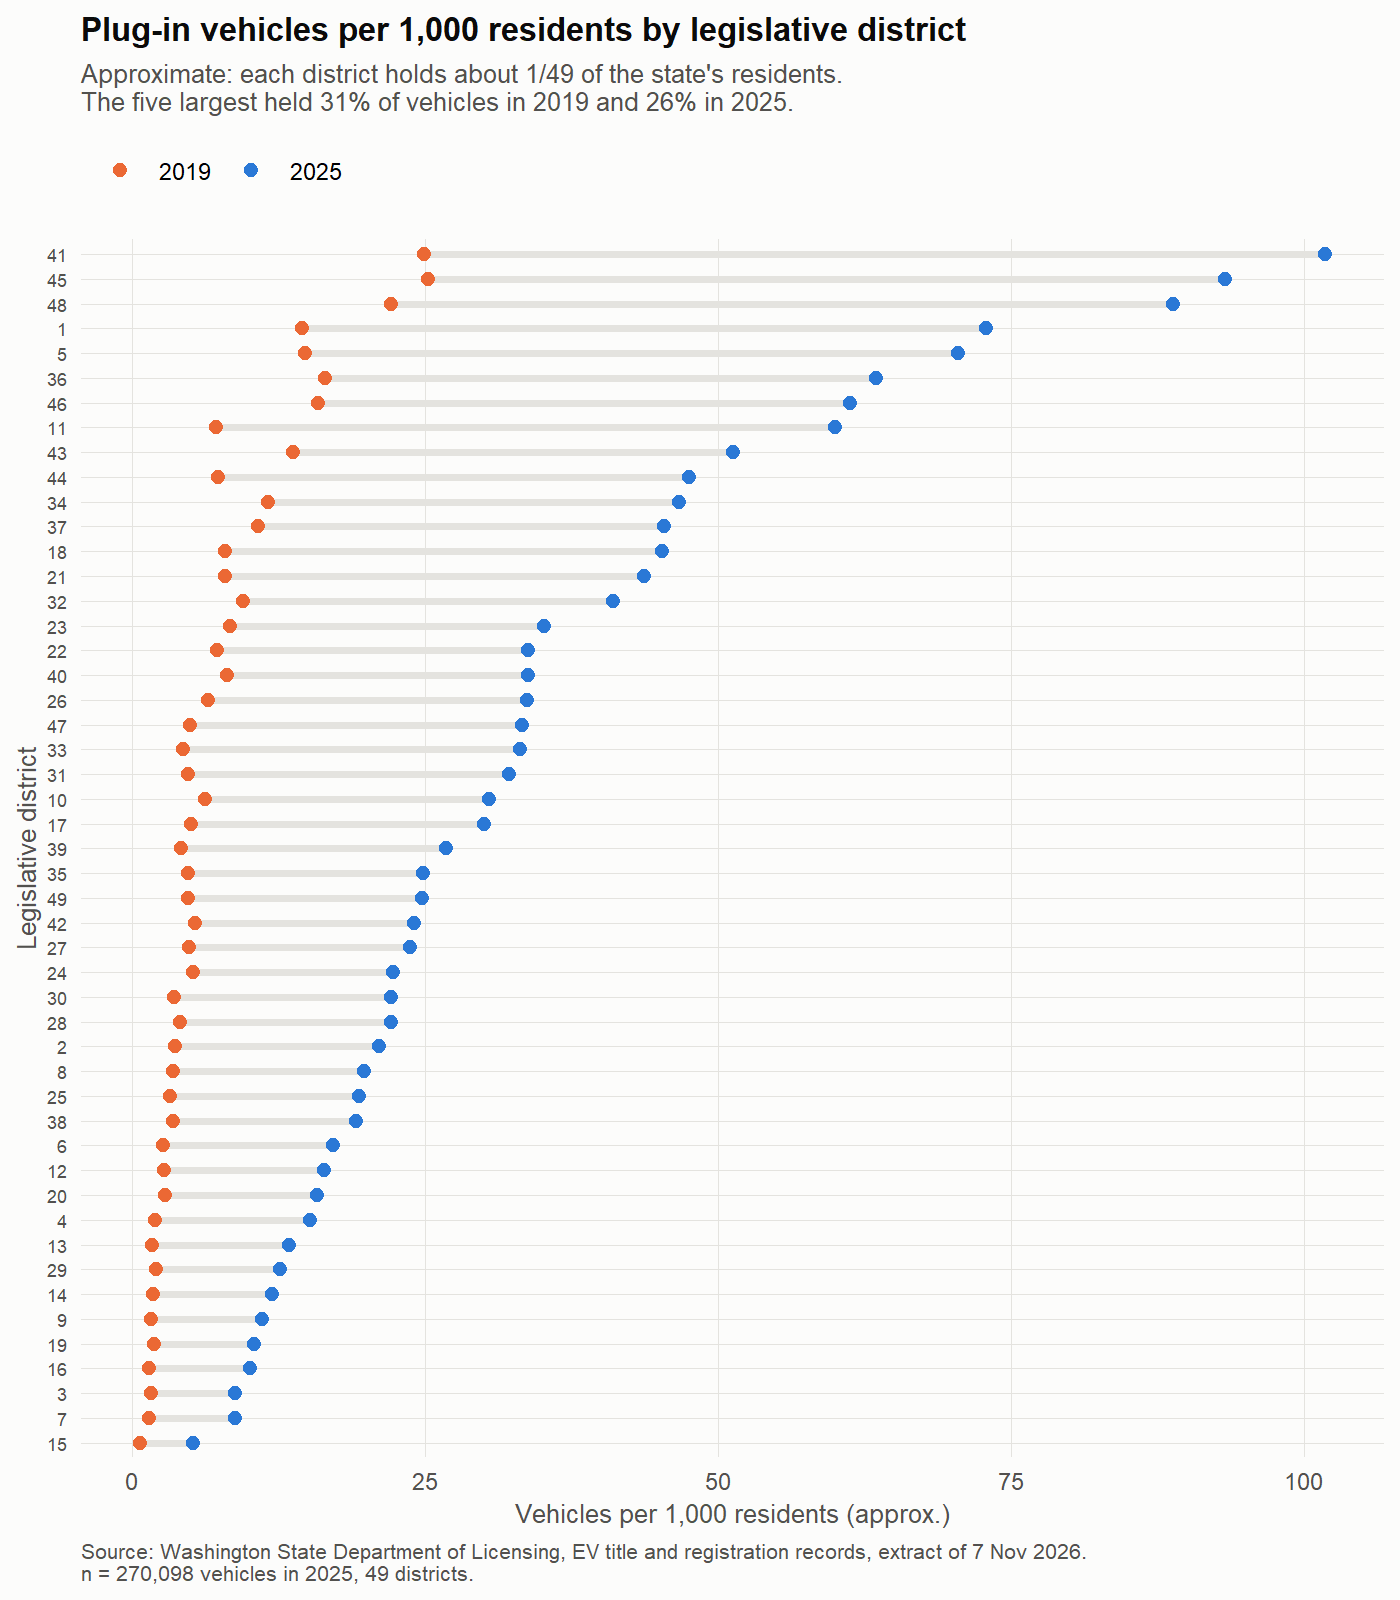
\includegraphics[width=6in,height=0.85\textheight,keepaspectratio]{21_01_districts_per_1000.png}
\caption{Vehicles per 1,000 residents by legislative district (21\_01\_districts\_per\_1000.png)}
\end{figure}

\begin{itemize}
  \item \textbf{Districts and utilities (ext. 7):} the five largest districts held 31\% of vehicles in 2019 and 26\% in 2025; districts 41, 45 and 48 have about 89--102 per 1,000 residents, district 15 about 5. Puget Sound Energy, Seattle and Tacoma territories hold 73\% of vehicles. code: 21.1--21.4.
\end{itemize}

\section{Actionable Conclusion and Insight}

\subsection{Key findings}

\begin{itemize}
  \item The population grew about five-fold from 2019 to 2025 (52,710 $\rightarrow$ 270,098) and is ageing (mean age 2.6 $\rightarrow$ 3.0 years).
  \item It is spreading: King's share fell 5.5 points, Eastern counties caught up on BEV share, and the top-five districts' share fell from 31\% to 26\%.
  \item Which vehicles stay: in the current fleet, BEVs and PHEVs leave at the same rate once age is taken into account (PHEVs stayed longer only before 2020); range shows no association. Leaving is associated with prior transfers, use class and region, and is hard to predict (AUC 0.57).
  \item About 7--7.5\% of active vehicles leave the records within two years (6.9\% from 2019, 7.5\% from 2023).
\end{itemize}

\subsection{Practical value}

\begin{itemize}
  \item \textbf{Planners and utilities:}
  \begin{itemize}
    \item charging and grid demand is concentrated (districts 41, 45, 48; 73\% of vehicles in three utility territories), but growth is now faster outside King --- plan new capacity there too.
    \item the projection (about 444,000 vehicles in 2028, with a wide interval) gives a range for load planning; update it each year as the 2026 check shows entries can shift quickly.
    \item per-resident rates (district 15 $\approx$ 5 per 1,000 vs 102 in district 41) identify under-served areas.
  \end{itemize}
  \item \textbf{State revenue and fleets:}
  \begin{itemize}
    \item EV registration fees depend on the active stock, not on sales: the stock-and-flow method (entries, a 7--7.5\% two-year exit rate, returns) is a transparent way to forecast that base.
    \item the end of the sales-tax exemption (July 2025) coincides with lower 2026 entries ($-11.8\%$); revenue planning should not assume the 2023--2025 entry level continues.
    \item fleet managers: BEVs and PHEVs now stay equally long, and used prices fall about 11\% per year of age --- useful for replacement and resale planning.
  \end{itemize}
  \item \textbf{Policy:}
  \begin{itemize}
    \item monitor equity: rural and eastern areas still have far fewer vehicles per resident.
    \item the records cannot say why a vehicle leaves; recording out-of-state transfers versus vehicles taken off the road would make retention measurable and models far stronger.
    \item publish population counts with the rules used (duplicates, exempt classes, two-year exit rule), because simple county sums double-count vehicles that move.
  \end{itemize}
\end{itemize}

\subsection{Limits and future research}

\begin{itemize}
  \item Associations, not causes; leaving is inferred from missing records; exits are only observable to 2023; 2025 is slightly provisional and 2026 partial.
  \item The projection holds rates constant and has one backtest origin; re-run it with later extracts.
  \item Future work: link with public charging-station data, out-of-state title transfers, and owner characteristics (not in this dataset).
\end{itemize}

\label{LastMainPage}

\includepdf[page=7-8]{../desc.pdf}

\end{document}
